\documentclass[11pt]{article}
\usepackage[margin=2cm,a4paper]{geometry}
\usepackage{graphicx}
\usepackage{authblk}
\usepackage{url}
\usepackage{array}
\usepackage{amsfonts}
\usepackage{multirow}
\usepackage{amsmath}
\usepackage[usenames, dvipsnames]{color, colortbl}
\usepackage[normalem]{ulem}
\usepackage{todonotes}
\usepackage[outdir=./img/]{epstopdf}
\usepackage{epsfig}

\usepackage{tikz}
\usetikzlibrary{fit,positioning}
\usetikzlibrary{arrows}

\makeatletter
\def\title#1{\gdef\@title{Supplement to: ``#1''}}
\makeatother
\renewcommand{\thetable}{S\arabic{table}}%
\renewcommand{\thefigure}{S\arabic{figure}}%
\renewcommand{\thepage}{S\arabic{page}}

\setlength\parindent{0pt}


% supplement referencing
\usepackage{subcaption}
%\usepackage{cleveref}

% tablet style table
 \usepackage{booktabs}
 
\title{Triqler for Protein Summarization of Data from Data Independent Aquisition Mass Spectrometry}
\author{Patrick Truong \and Matthew The \and Lukas K\"{a}ll}


\begin{document}

\maketitle

\section*{Note S1: Supplementary figures and tables}
\label{sec:fc-eval}


\begin{table}[hbt]
\centering
\begin{tabular}{lll}
\hline
        & Unfiltered & no\_shared \\ \hline
All     & 31 055     & 30 456     \\
E. Coli & 4 391      & 4 306      \\
Human   & 20 614     & 20 302     \\
Yeast   & 6 050      & 5 848      \\ \hline
\end{tabular}

  \caption{{\bf Protein count in the Uniprot FASTA protein database.} The database is a FASTA file with one protein sequence per gene for each species (UP000005640, UP000000625, and UP000002311. Acquired on 2021-06-16). We further filtered the sequences to assure that no two proteins shared tryptic peptides longer than 7 amino acids. The number of sequences remaining after this operation is reported in the no\_shared column. \label{table:proteins_in_database}}

\end{table}



\begin{table}[h]
    \begin{tabular}{l|lll|lll}
    \hline
    \multicolumn{7}{c}{ID workflow} \\ \hline
    Condition & \multicolumn{3}{c|}{A} & \multicolumn{3}{c}{B}\\
    \hline
    Filename       & 002-Pedro & 004-Pedro & 006-Pedro & 003-Pedro & 005-Pedro & 007-Pedro \\
    \hline
    Peptides  & 12 934                        & 13 819                        & 13 063                        & 12 023                        & 14 858                        & 15 208                        \\
    Proteins  & 2 252                         & 2 321                         & 2 243                         & 2 159                         & 2 427                         & 2 433                         \\ \hline
    \end{tabular}
     \caption{{\bf Number of identified peptides and proteins for the ID workflow.} A peptide-level FDR at 0.01 was obtained using a an $m\_score$ cutoff at 0.00079 computed by setting the desired peptide-level FDR with \texttt{mscore4pepfdr} in the \texttt{SWATH2stats} package.
          \label{fig:osw_peptide_and_protein_id}}
    \todo[inline]{At which FDR thresholds?}
\end{table}
        

\begin{table}[h]
    \begin{tabular}{l|lll|lll}
    \hline
    \multicolumn{7}{c}{PS workflow}                                                                                                                                                                                   \\ \hline
    Condition & \multicolumn{3}{c|}{A}                                                                         & \multicolumn{3}{c}{B}                                                                         \\
    \hline
    Filename       & 002-Pedro & 004-Pedro & 006-Pedro & 003-Pedro & 005-Pedro & 007-Pedro \\
    \hline
    Peptides  & 20 880                        & 20 653                        & 20 907                        & 21 118                        & 21 192                        & 21 137                        \\
    Proteins  & 3 228                         & 3 224                         & 3 240                         & 3 243                         & 3 255                         & 3 249                         \\ \hline
    \end{tabular}
     \caption{{\bf Number of identified peptides and proteins for the PS workflow} A peptide-level FDR at 0.01 was used for the purpose of reporting these figures.
          \label{fig:diann_peptide_and_protein_id}}
          \todo[inline]{At which FDR thresholds?}
\end{table}


\begin{figure}[hbt]
    \centering
    \centering
    \begin{tabular}{lclc} 
        A & 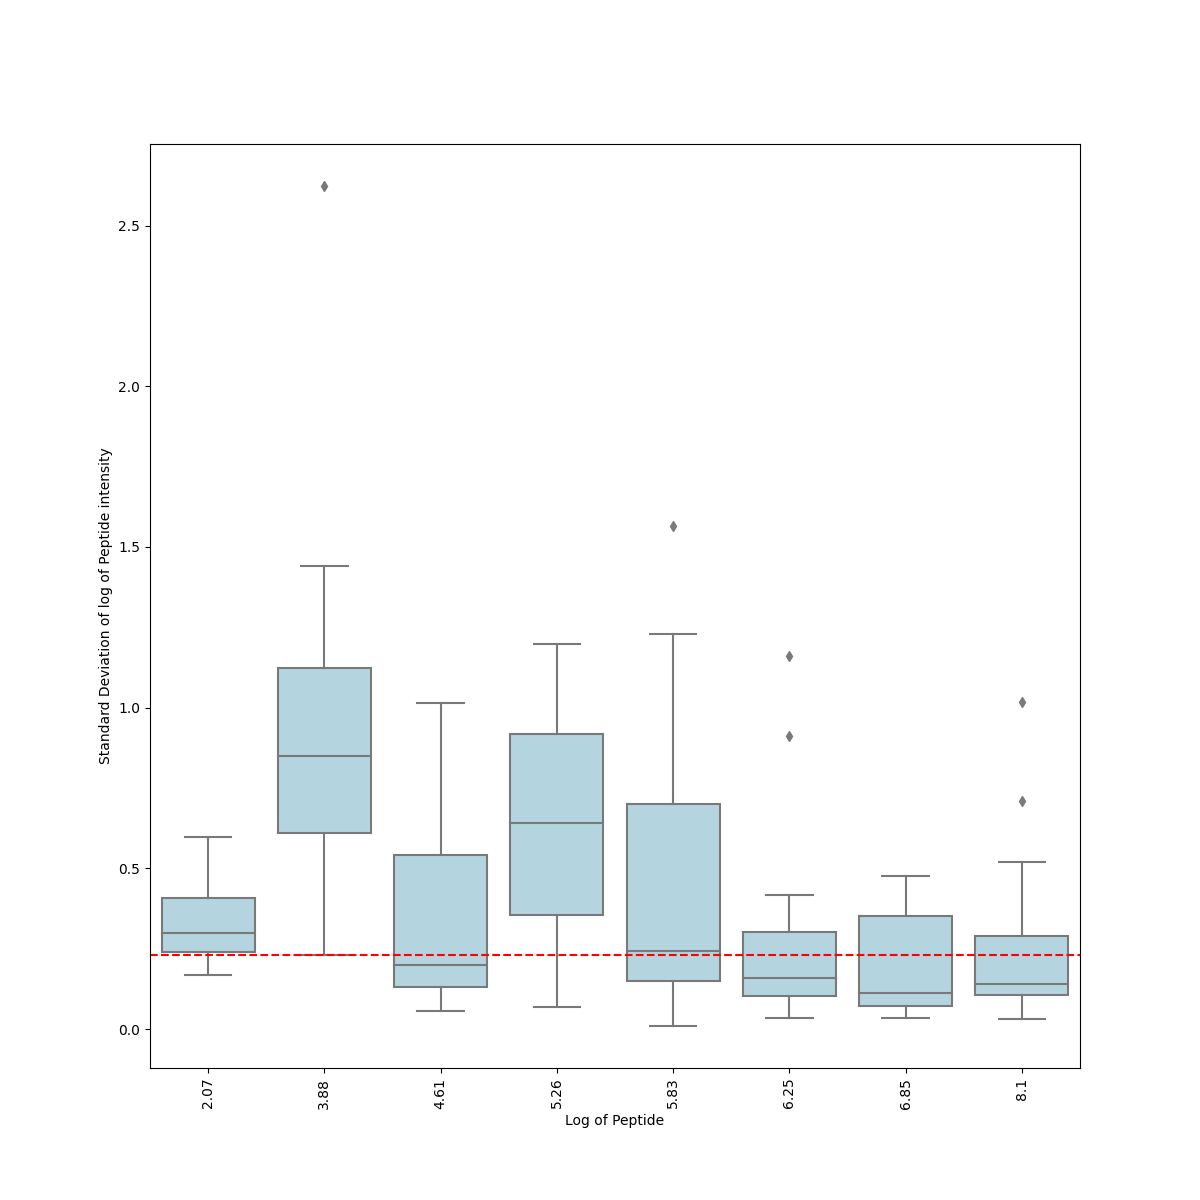
\includegraphics[width=0.4\linewidth]{../../result/report_plots_pipeline/quantile_bins_ID_median.png} &
        B & 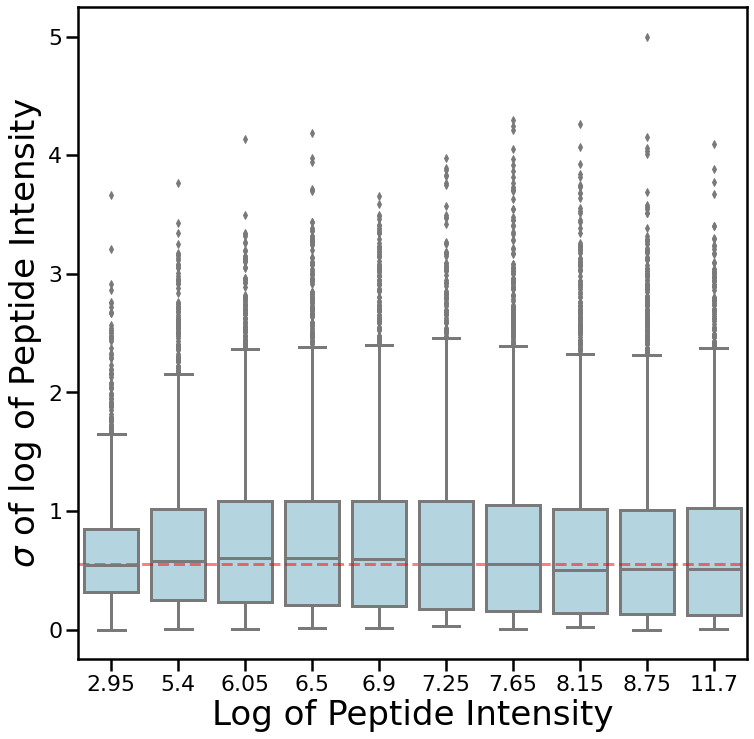
\includegraphics[width=0.4\linewidth]{../../result/report_plots_pipeline/quantile_bins_PS_median.png} \\
    \end{tabular}
  \caption{{\bf Standard deviation of peptide abundance as a function of mean abundance in DIA experiments.} We performed quantile binning with 10 bins using pandas qcut function and plotted the standard deviation across samples as a function of the mean of every peptide intensity in the TripleTOF6600 section of the LFQ Bench set. The bins are constructed so that each bin contains an equal amount of data points and the unequal bin sizes are an effect of the quantile binning procedure. The x-axis value shows the bin ranges. We used a log-log scale for abundances derived by the (A) ID pipeline and (B) PS pipeline. (A) show a slight increase in peptide intensity standard deviation as we increase the mean peptide intensity. In (B) we observe a nearly uniform offset in standard deviation across the intensity scale, demonstrating that (B) holds the Triqler assumption $\log(\sigma) \approx \log(\mu) + \log(k)$ and hence   $\sigma \approx \mu k$ very well. While (A) does not hold the assumption as well, Triqler is still used to analyse this data.  \label{fig:uniform_offset_in_standard_deviation_boxplot}}

 \end{figure}
 

\begin{figure}[hbt]
    \centering
    \centering
    \begin{tabular}{lclc} 
        A & 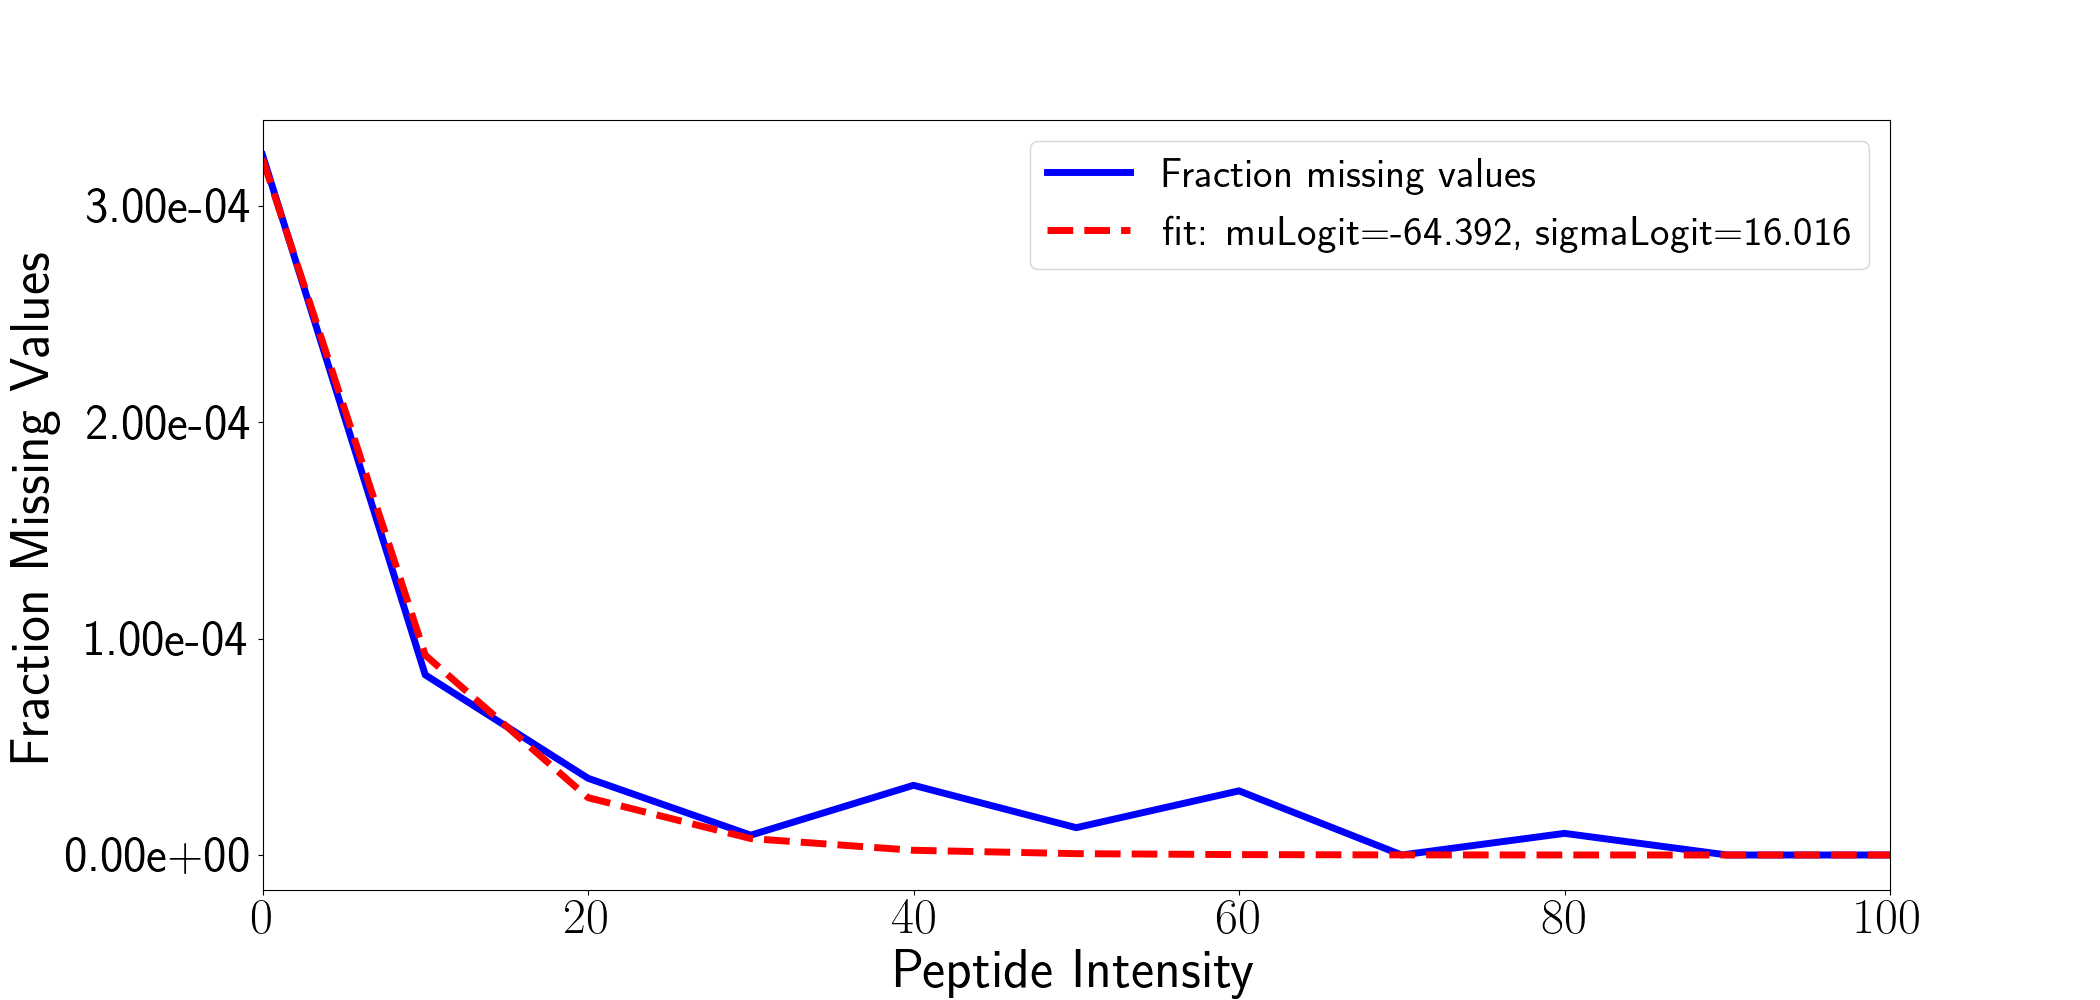
\includegraphics[width=0.80\linewidth]{../../result/report_plots_pipeline/fraction_missing_values_ID.png} \\ %\includegraphics[width=0.3\linewidth]{} & 
        B & 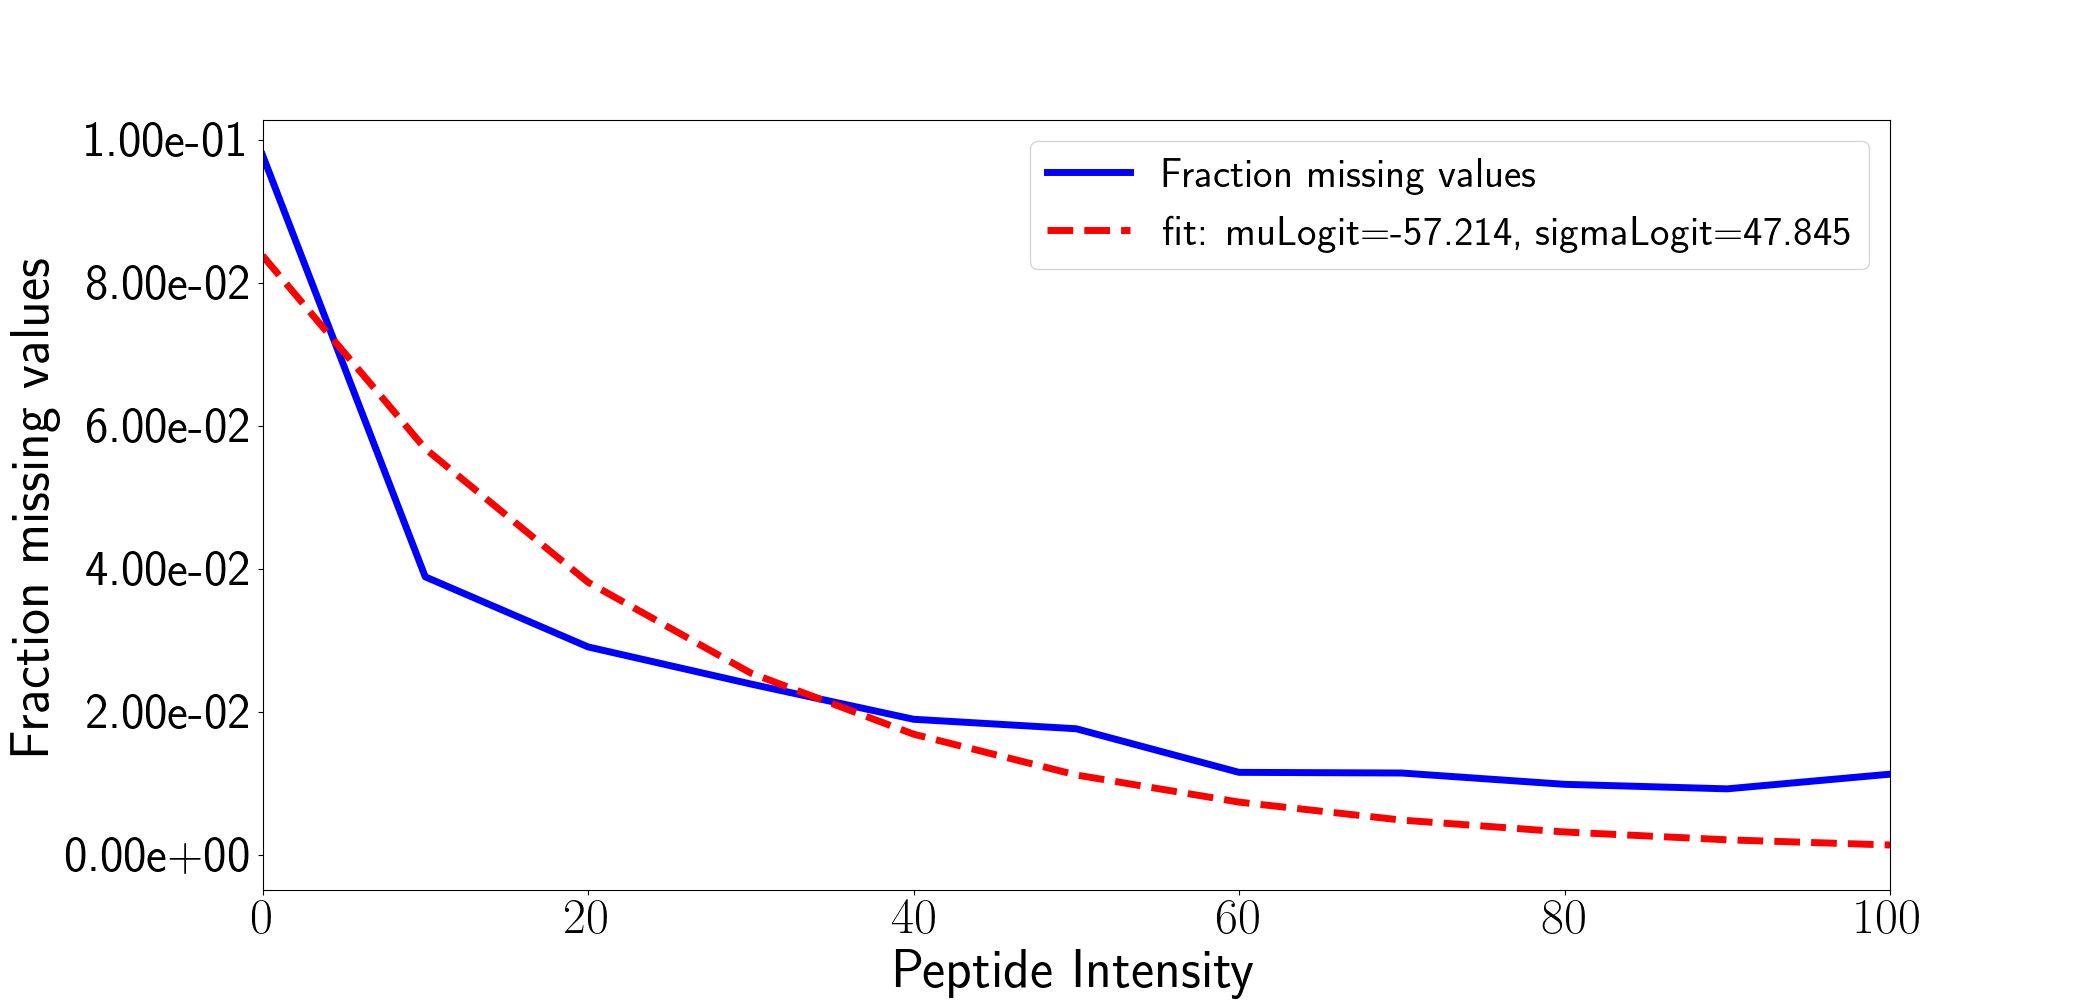
\includegraphics[width=0.80\linewidth]{../../result/report_plots_pipeline/fraction_missing_values_PS.png} \\%\includegraphics[width=0.3\linewidth]{} \\ 
    \end{tabular}
    \caption{{\bf Comparison of actual missing values against fit to the censored normal distribution used in Triqler.} We imputed the missing values as the mean of sample peptide intensities and used these imputed values to approximate the missingness for a given intensity. We binned the intensities to an arbitrary small range and plotted the fraction of missing values for each intensity range. The curve\_fit function from scipy.optimize was used to fit the values against the mentioned censored normal distribution for (A) ID pipeline  and (B) PS pipeline. \label{fig:fraction_missing_values}}
\end{figure}

\begin{figure}[hbt]
    \centering
    \centering
    \begin{tabular}{lclc} 
        A & 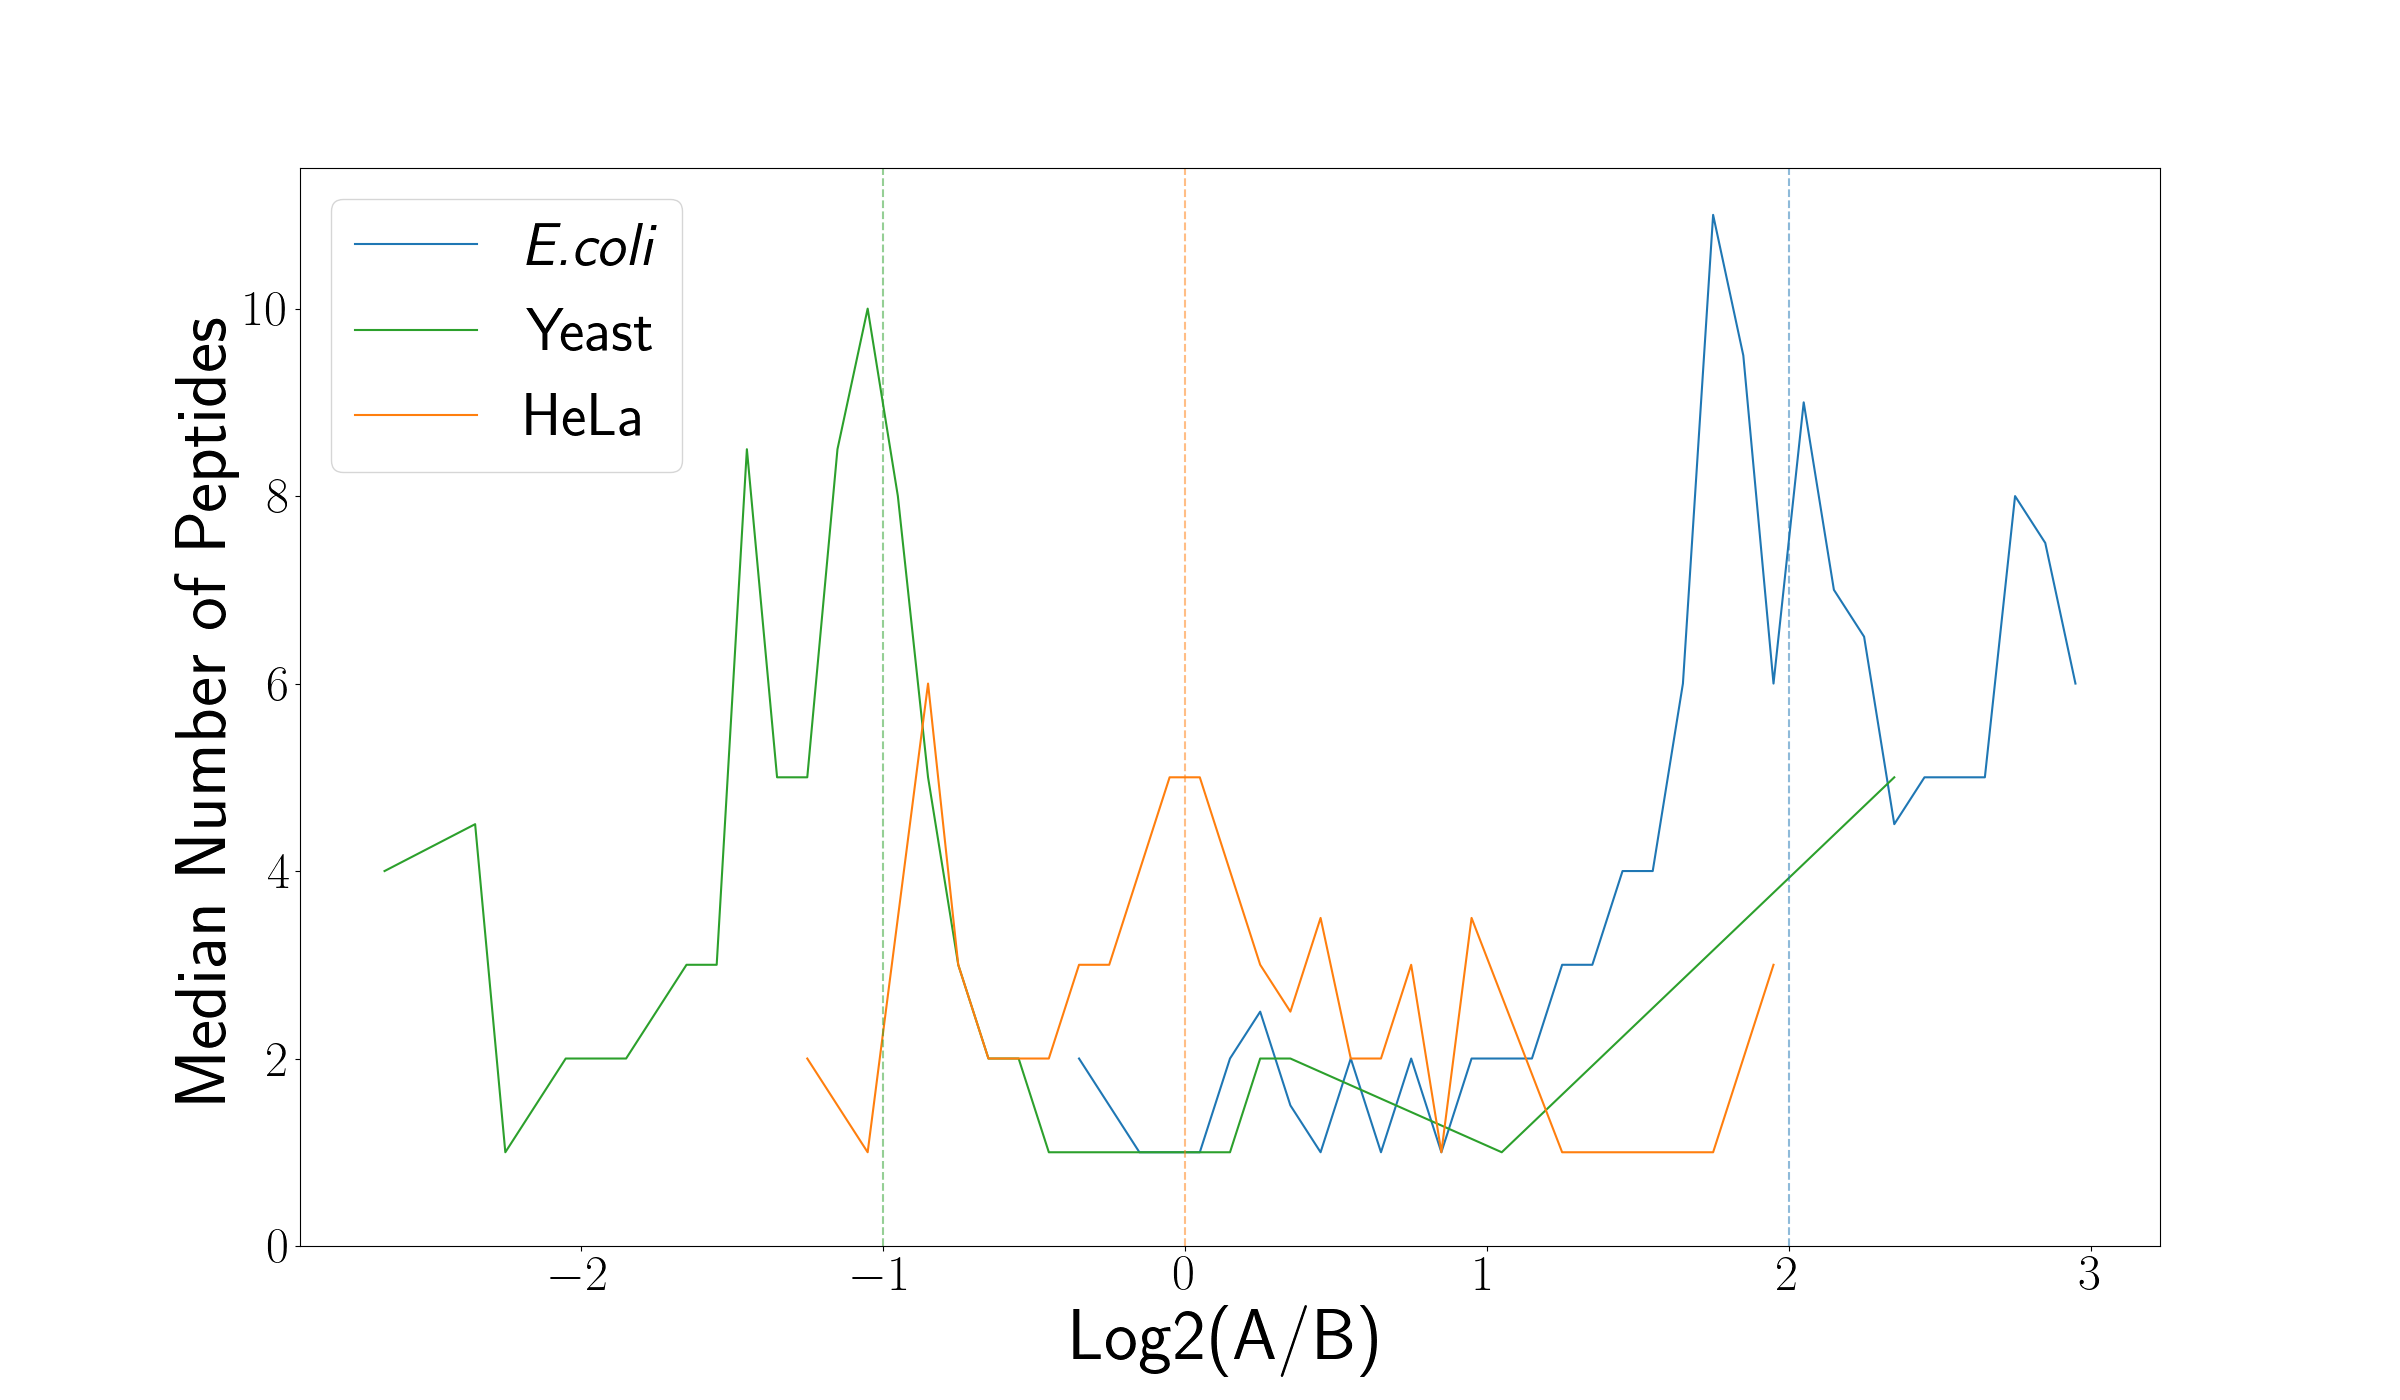
\includegraphics[width=0.5\linewidth]{../../result/report_plots_pipeline/fc_peptide_count_ID_triqler.png} &
        B & 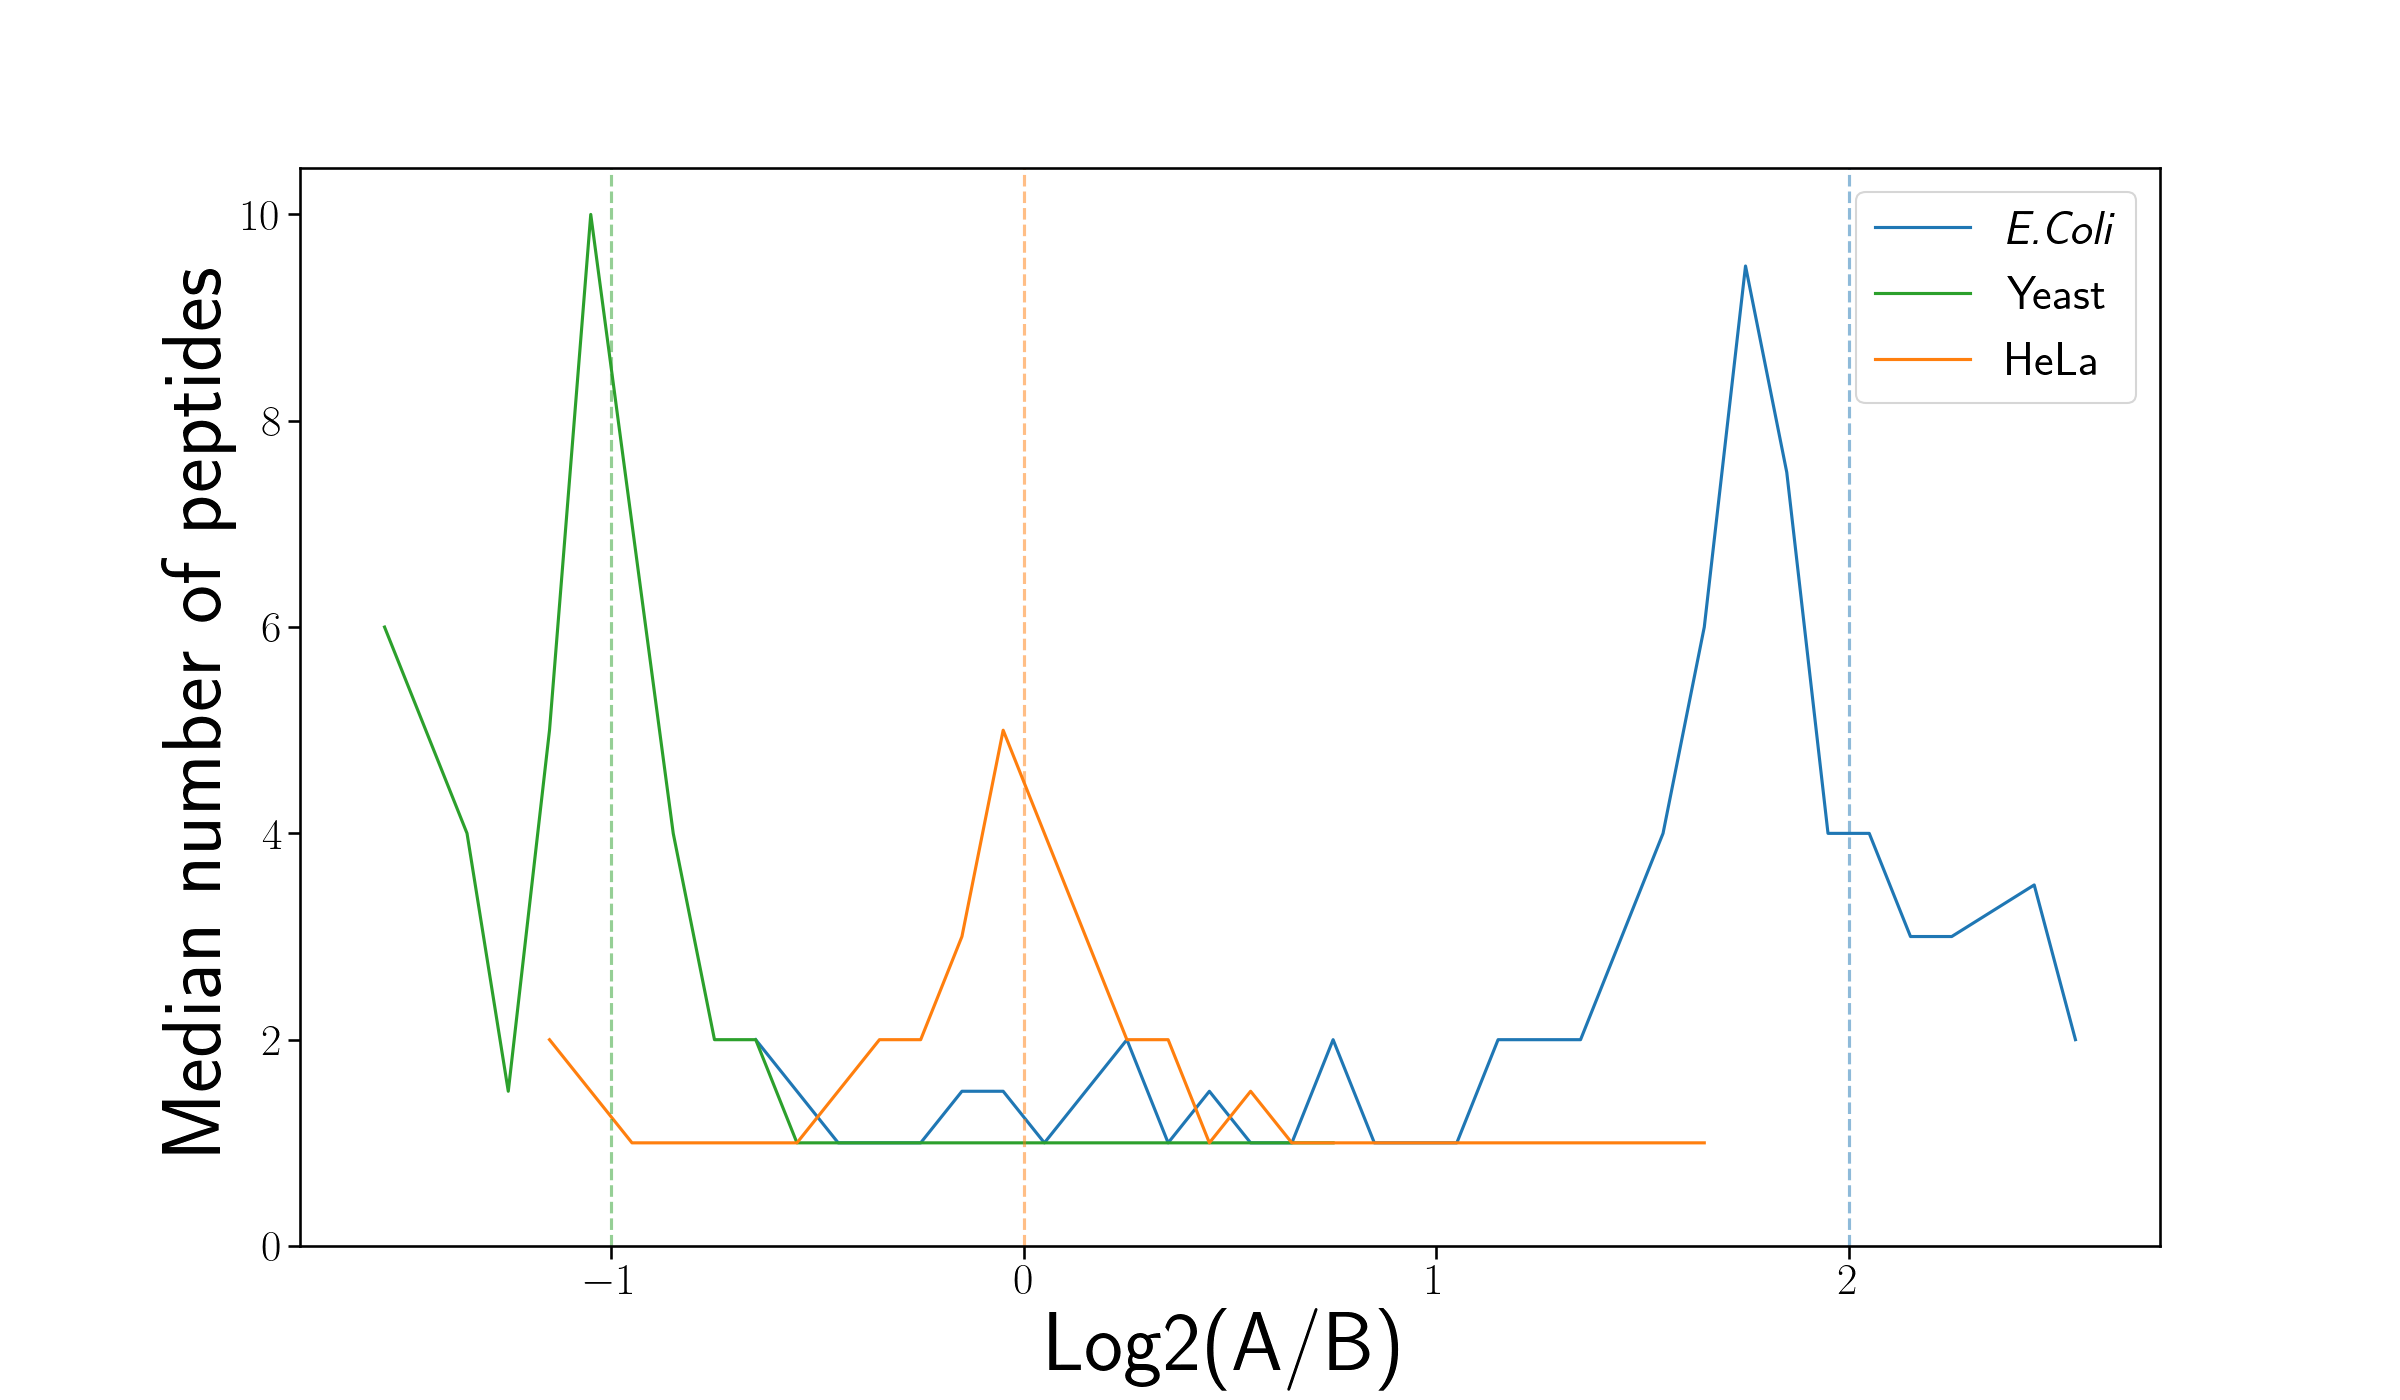
\includegraphics[width=0.5\linewidth]{../../result/report_plots_pipeline/fc_peptide_count_PS_triqler.png} \\
    \end{tabular}
    \caption{{\bf Proteins with a different Triqler-estimated abundance than expected are summarized by fewer peptides than ones that are well estimated.} We plotted the median number of peptides per protein for    
  We binned the peptides into regions of 0.1 ranged bins of estimated fold change and plotted them median for all bins between [-2,3], and plotted the median number of peptides as a function of bin-centers of the fold change. (A) is the ID pipeline and (B) is the PS pipeline \label{fig:number_of_peptides_supplement}}
  \todo[inline]{I still not sure what to get from this plot. It might be interesting to show that there is a difference in triqler as compared to other methods in this aspect, is that something we should claim? }
\end{figure}

\begin{figure}[hbt]
    \centering
    \newcolumntype{V}{>{\centering\arraybackslash} m{.4\linewidth} }
    \setlength{\tabcolsep}{0pt}
   %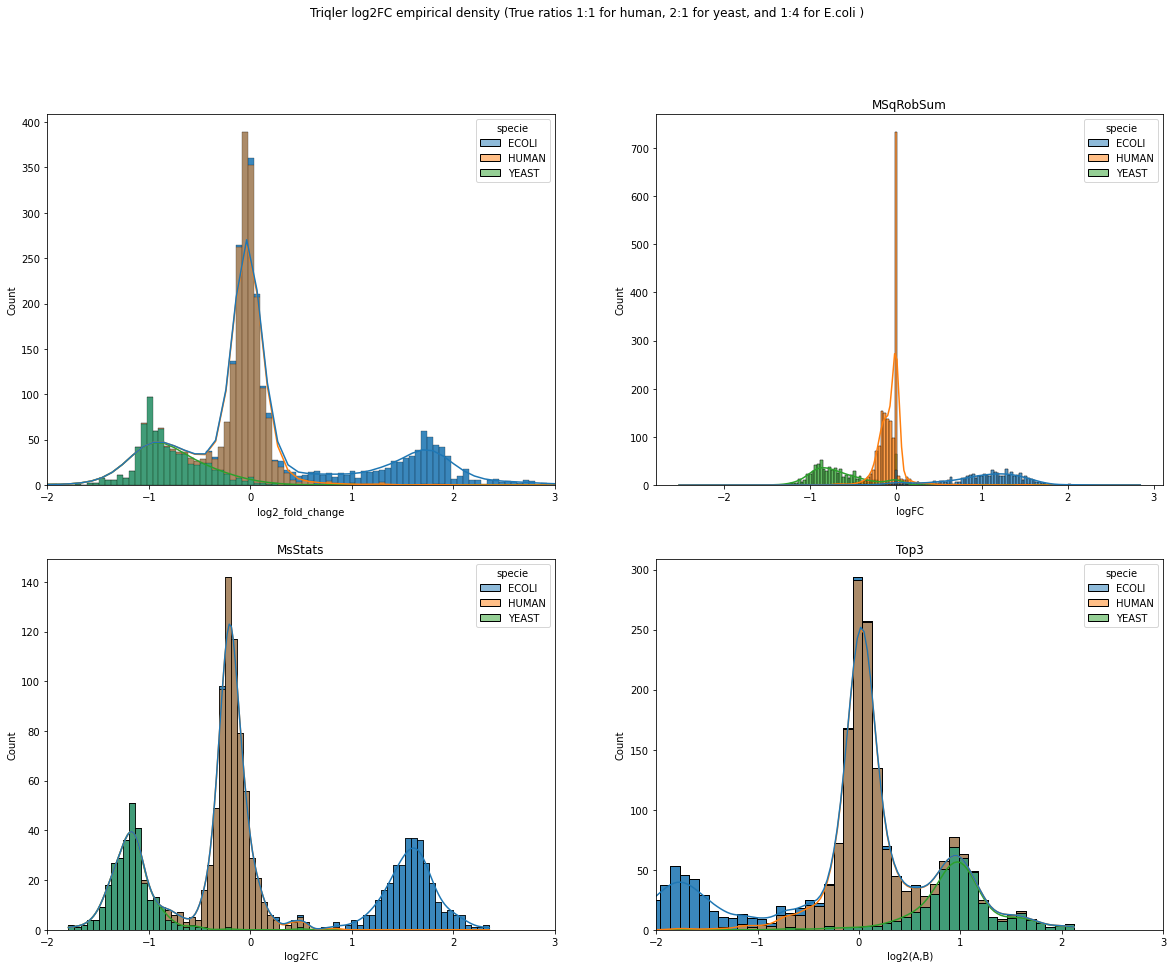
\includegraphics[width=16cm]{../../result/2021-08-13_docs_plots/intensity_plot.png}
    \begin{tabular}{   >{\centering\arraybackslash} m{3cm} V V}
                & ID & PS \\
        {\rotatebox[origin=c]{90}{Triqler vs Top3}} & 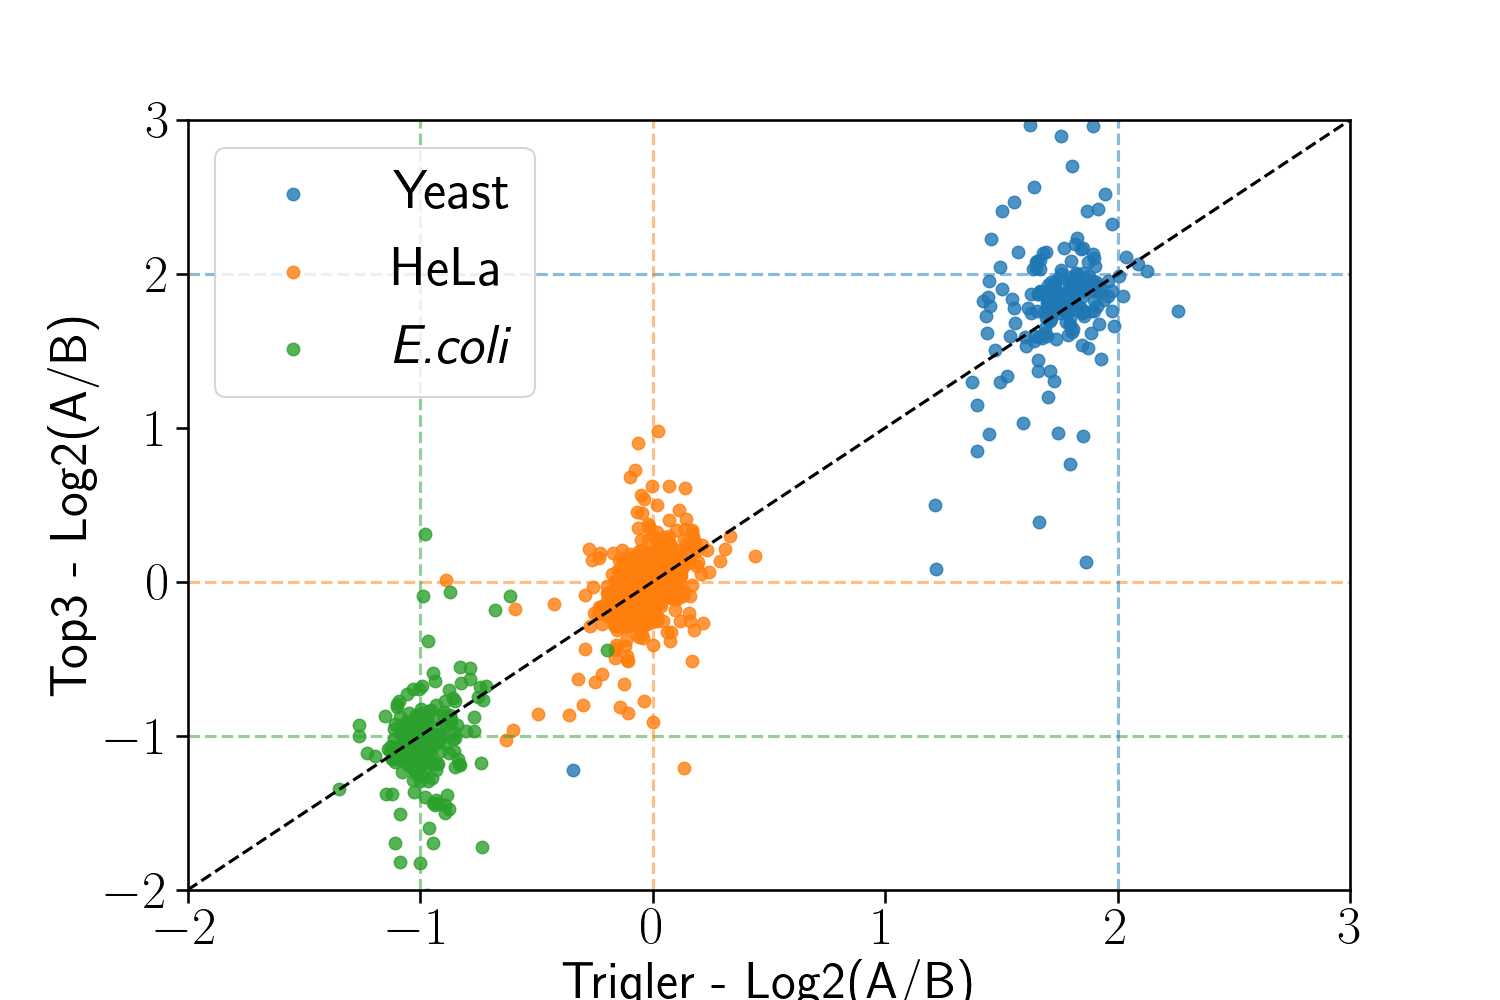
\includegraphics[width=\linewidth]{../../result/report_plots_pipeline/scatter_ID_triqler_vs_top3.png}  
                & 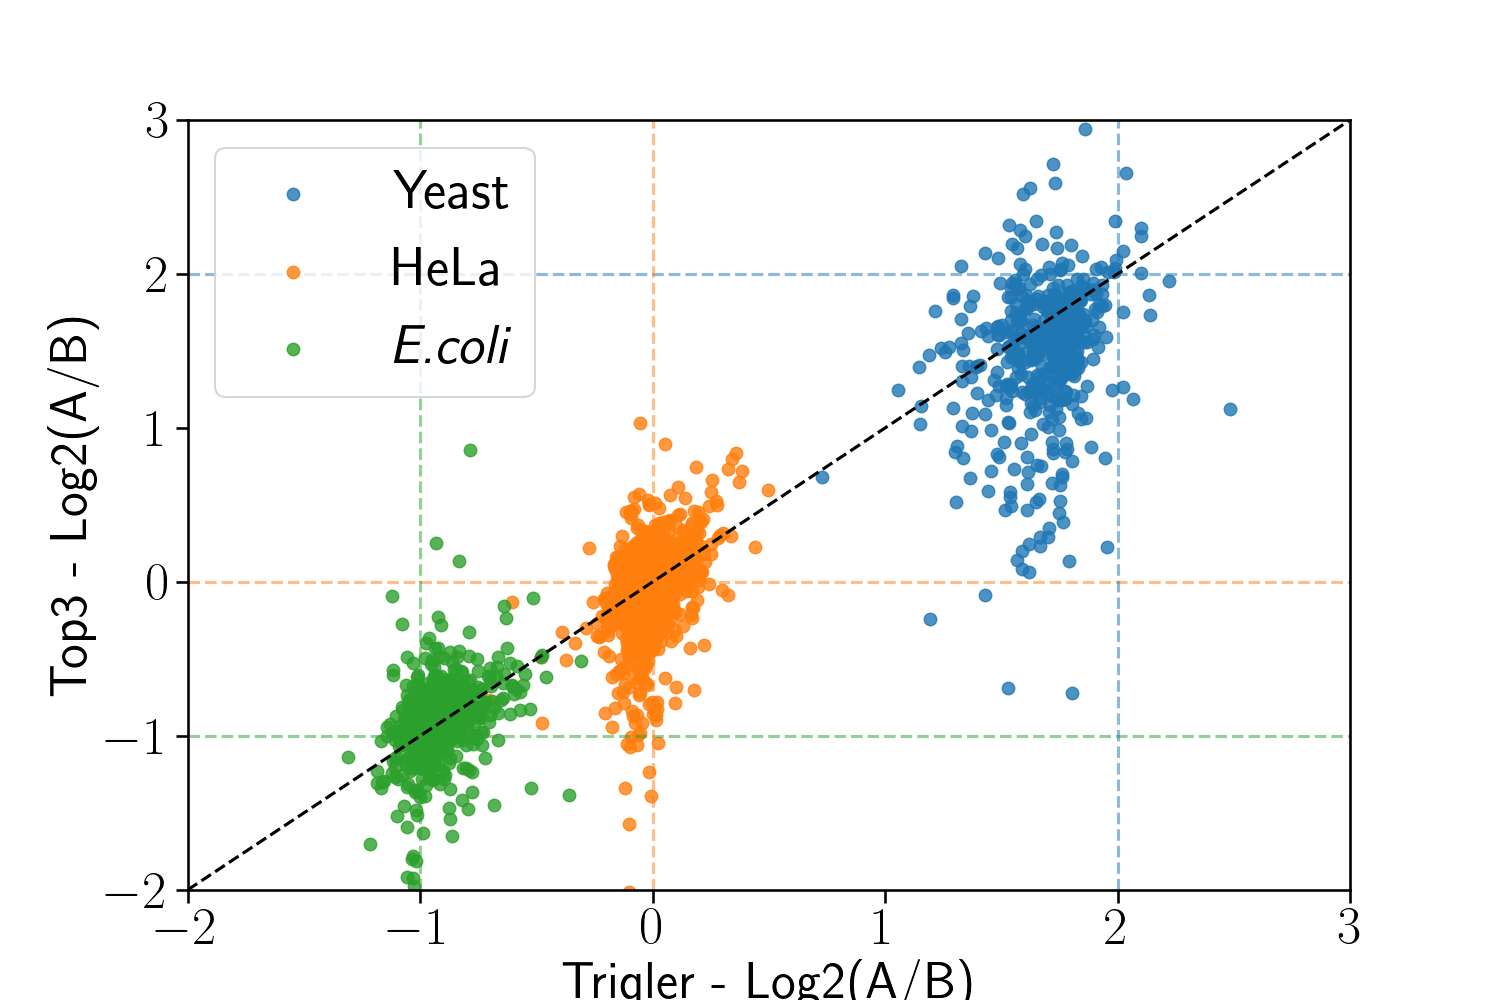
\includegraphics[width=\linewidth]{../../result/report_plots_pipeline/scatter_PS_triqler_vs_top3.png} \\ 
        {\rotatebox[origin=c]{90}{Triqler vs MSstats}} & 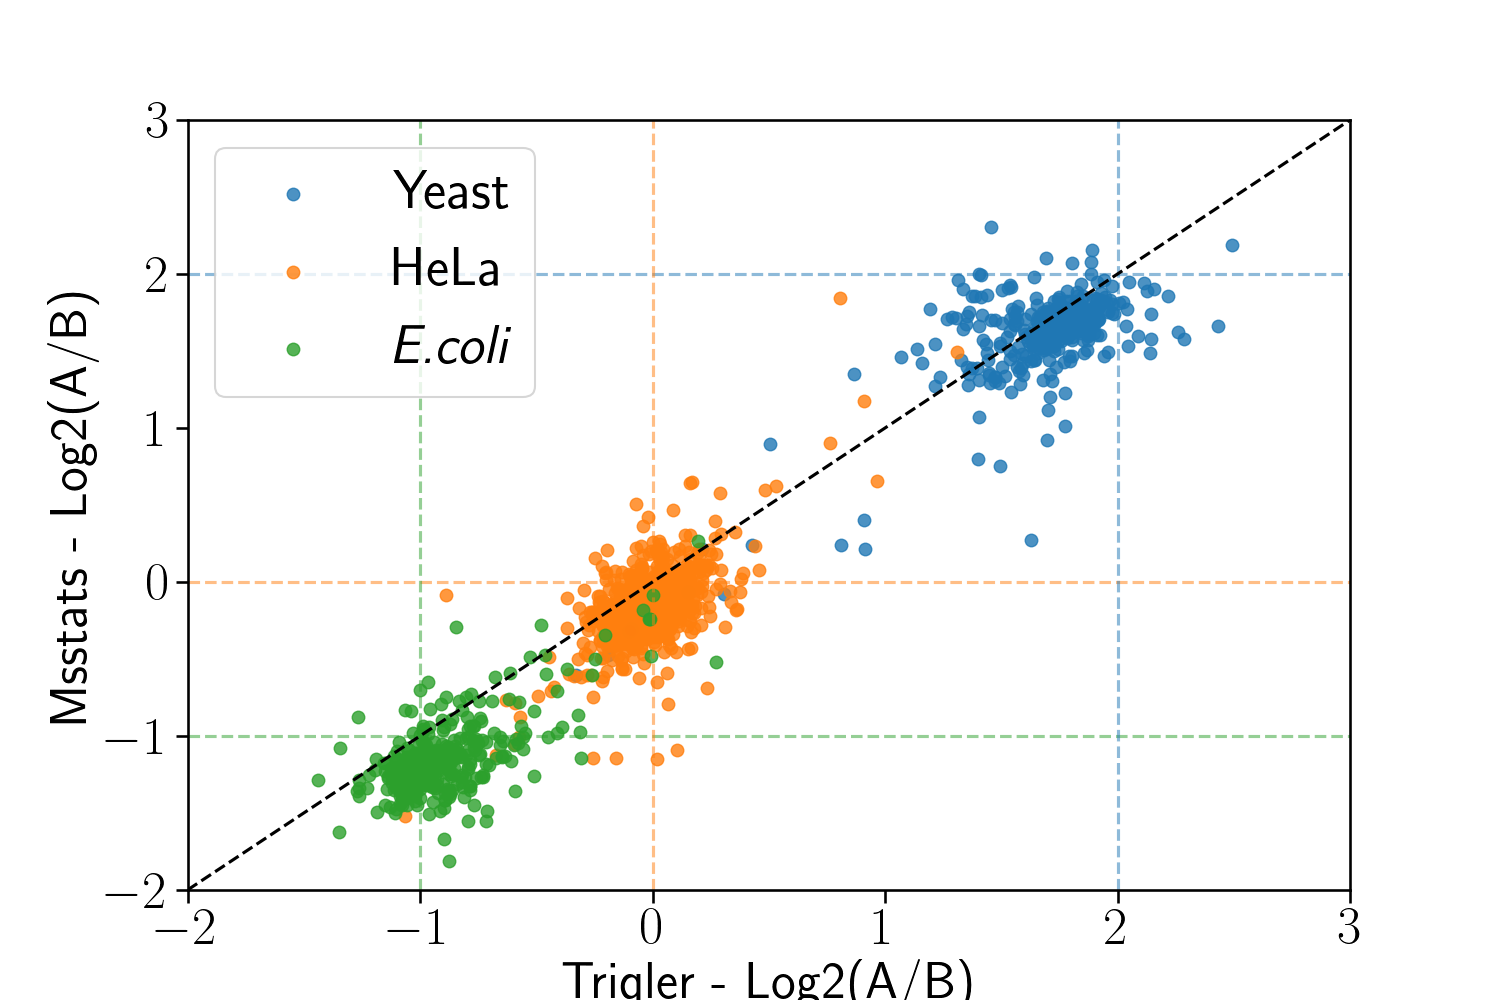
\includegraphics[width=\linewidth]{../../result/report_plots_pipeline/scatter_ID_triqler_vs_msstats.png}  
                & 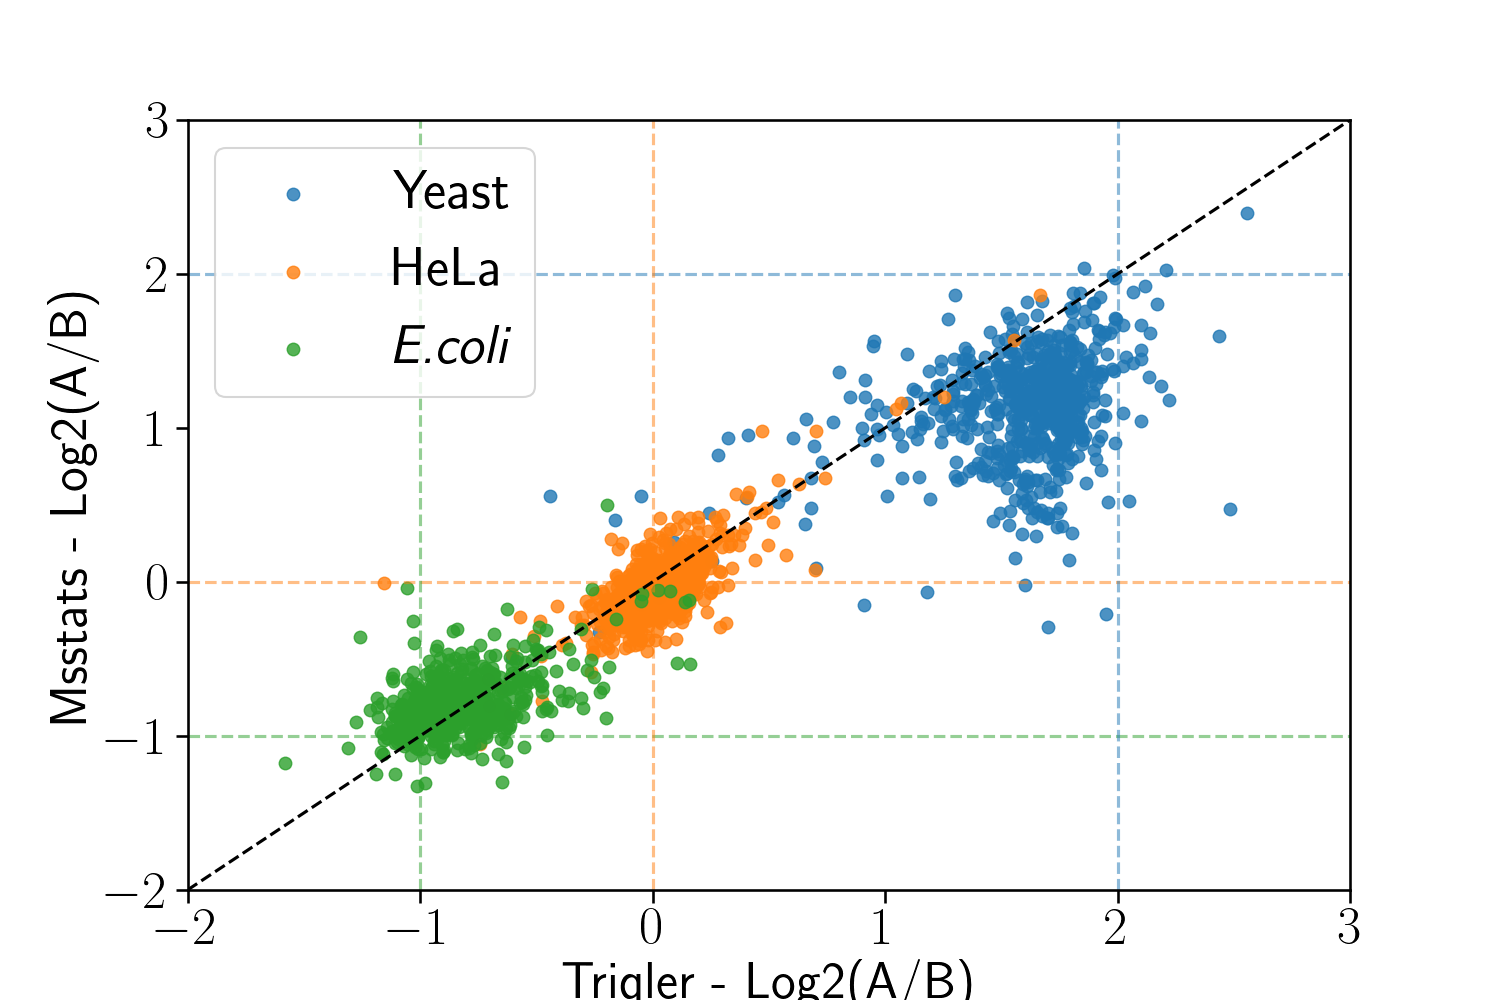
\includegraphics[width=\linewidth]{../../result/report_plots_pipeline/scatter_PS_triqler_vs_msstats.png} \\ 
        {\rotatebox[origin=c]{90}{Triqler vs MSqRob2}} & 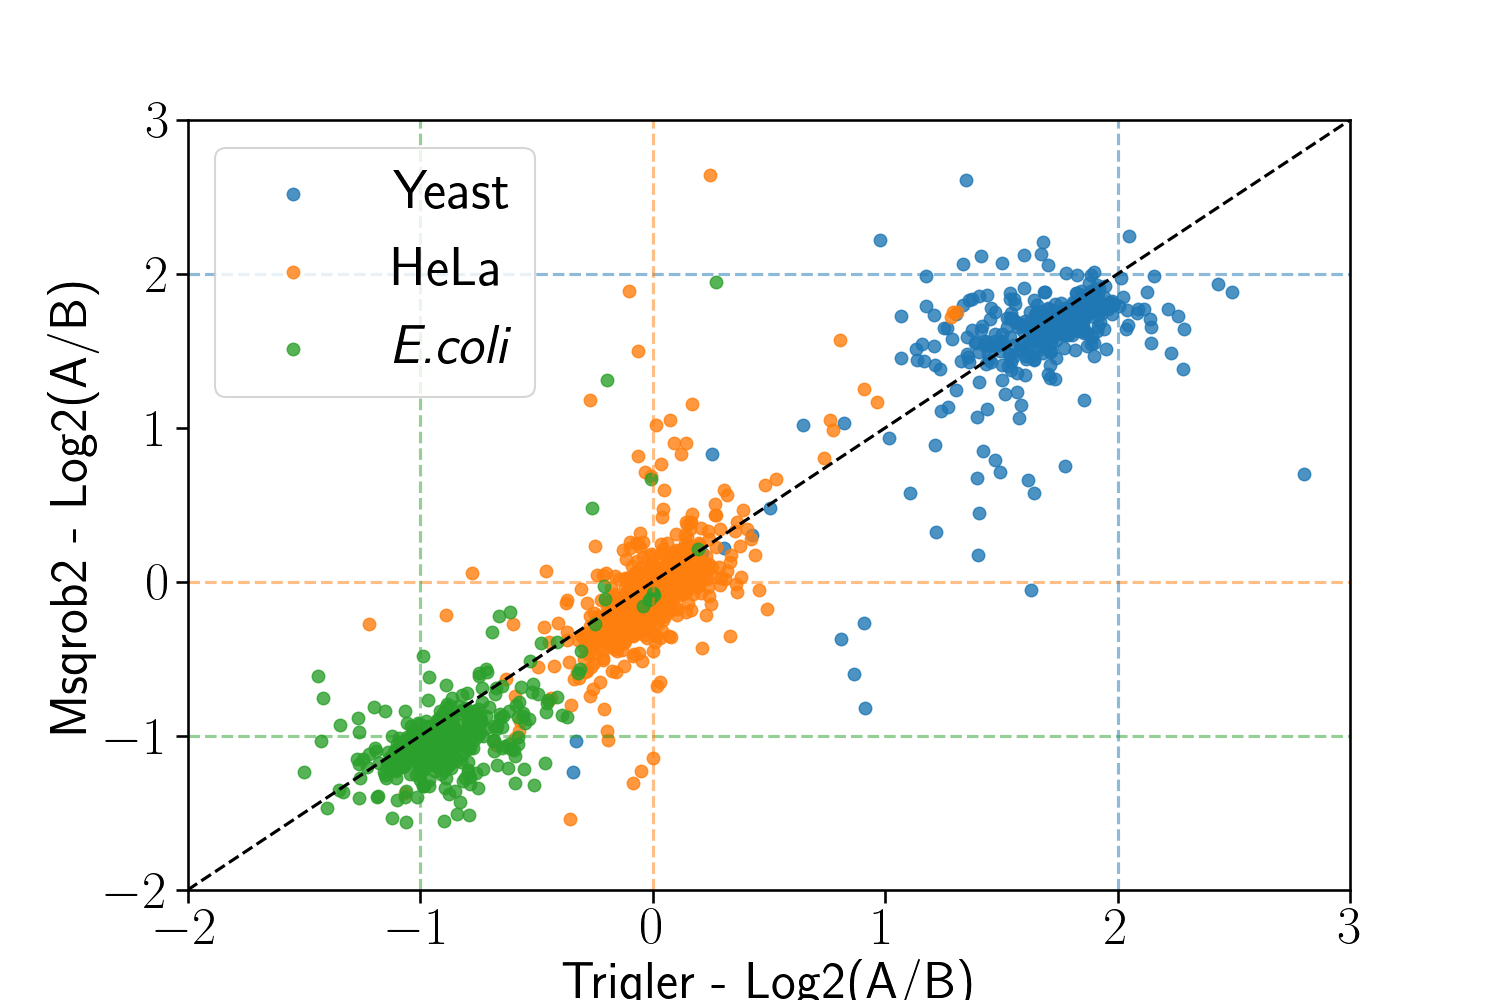
\includegraphics[width=\linewidth]{../../result/report_plots_pipeline/scatter_ID_triqler_vs_msqrob2.png}  
                & 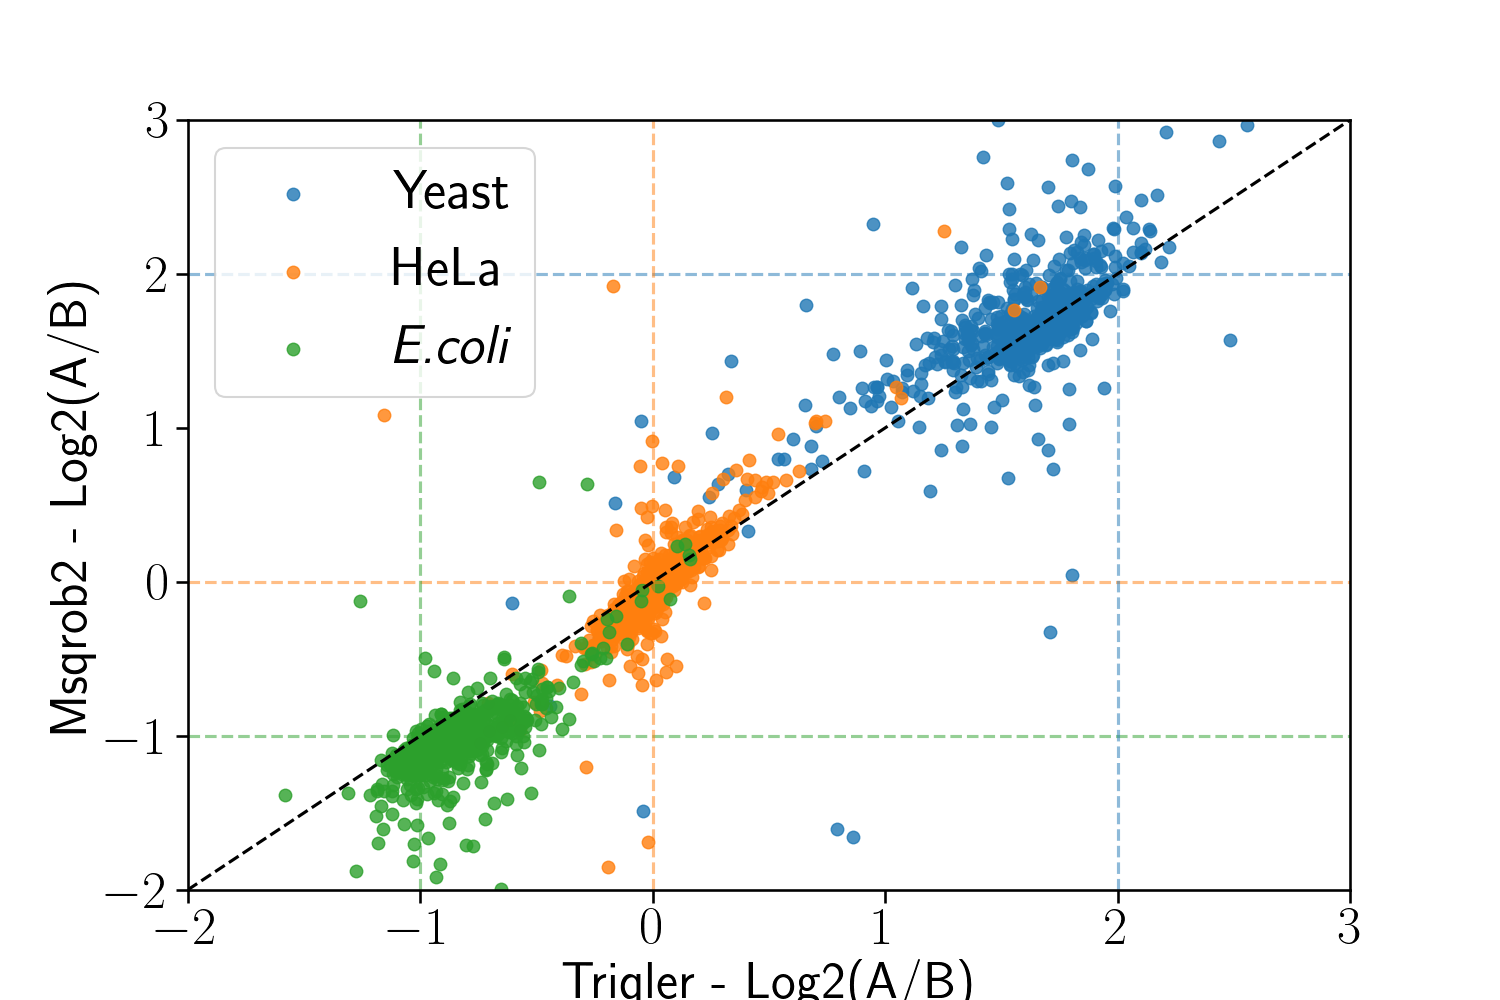
\includegraphics[width=\linewidth]{../../result/report_plots_pipeline/scatter_PS_triqler_vs_msqrob2.png} \\ 
    \end{tabular}
    \caption{{\bf Comparison of reported log2-fold change between Triqler and the compared methods.} from ID and PS pipelines. Top3 proteins have a higher variance in log2-fold changes than Triqler. MSstats and MSqRob2 has a bias for the \textit{E. coli} group. \label{fig:fc_scatter_triqler_vs_method_supplement}}
   
\end{figure}


\begin{figure}[hbt]
    \centering
    \begin{tabular}{lclc} 
        A & 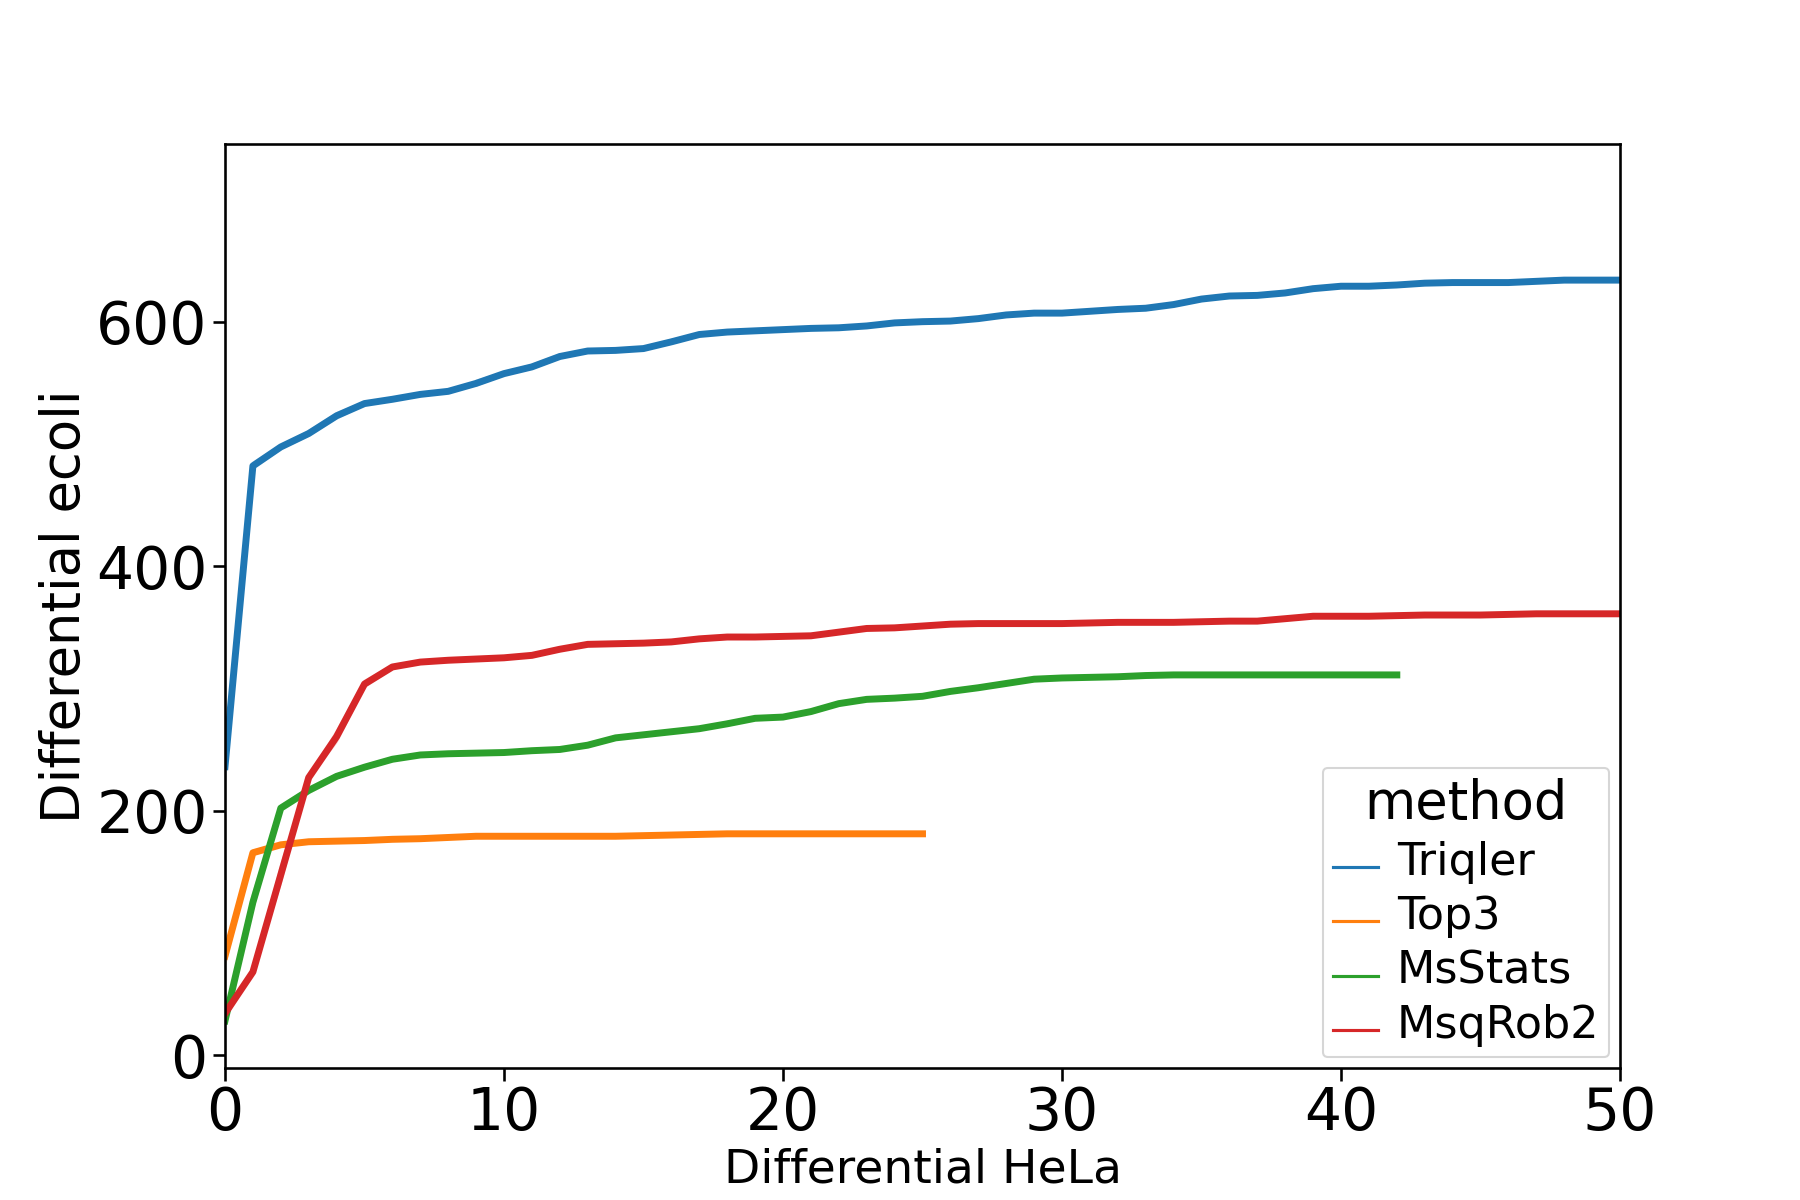
\includegraphics[width=0.4\linewidth]{../../result/report_plots_pipeline/diff_HeLa_vs_nonHeLa_ID_ecoli_0.51.png} & 
        D & 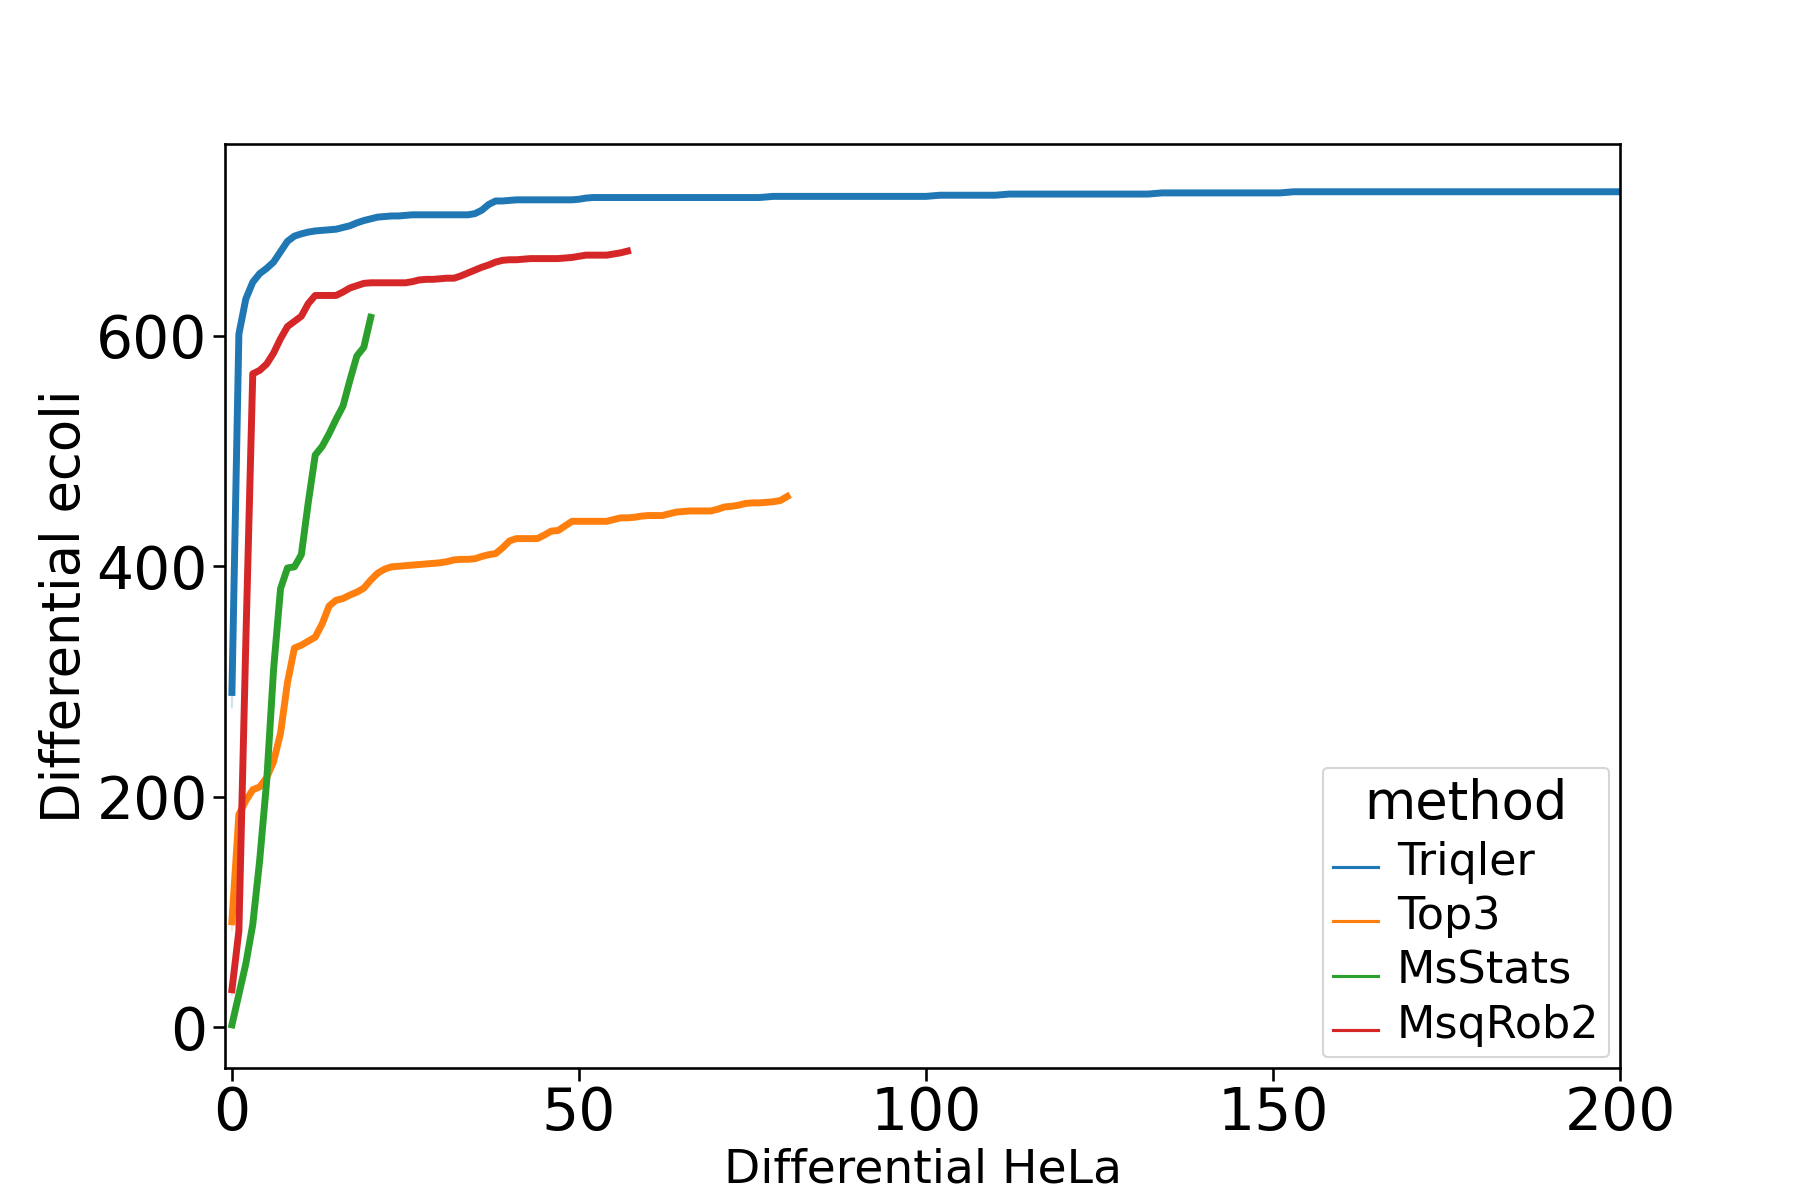
\includegraphics[width=0.4\linewidth]{../../result/report_plots_pipeline/diff_HeLa_vs_nonHeLa_PS_ecoli_0.51.png} \\ 
        B & 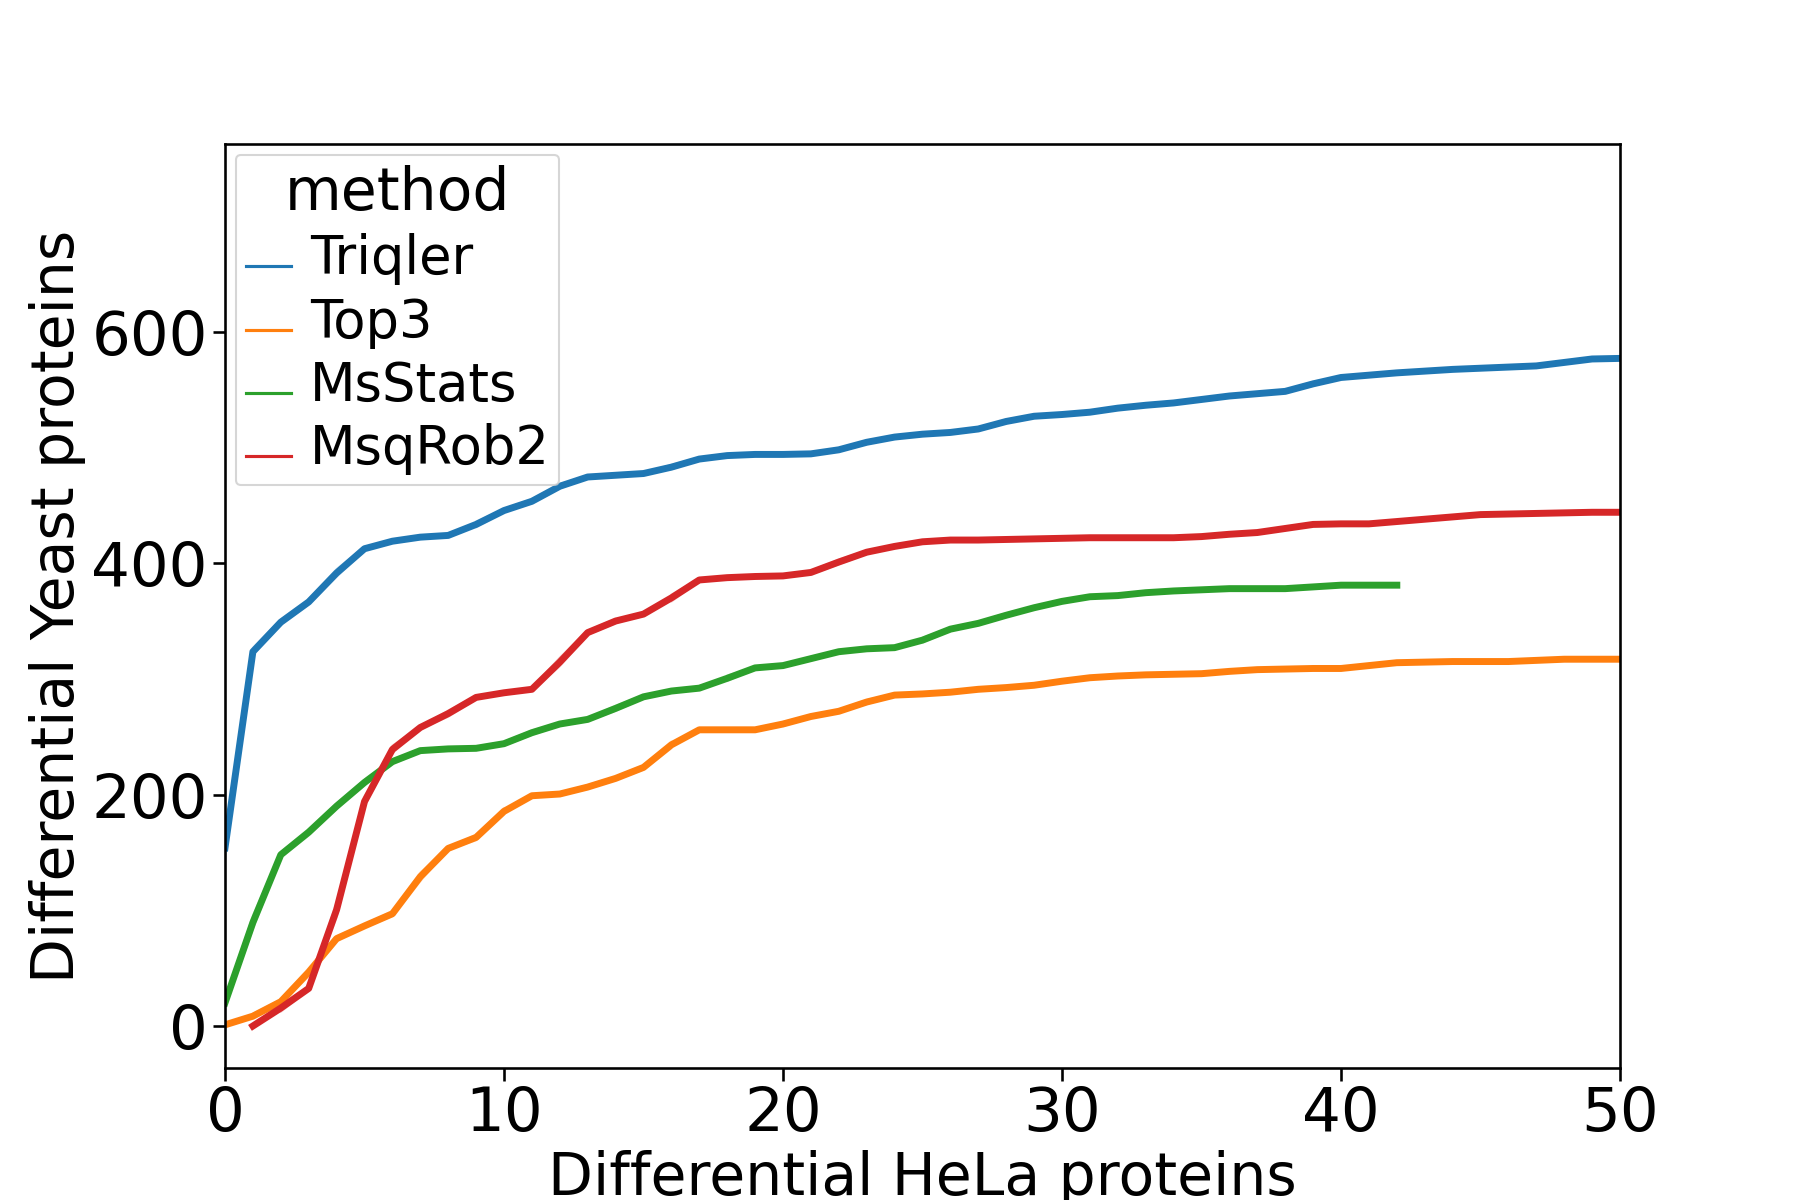
\includegraphics[width=0.4\linewidth]{../../result/report_plots_pipeline/diff_HeLa_vs_nonHeLa_ID_yeast_0.51.png} & 
        E & 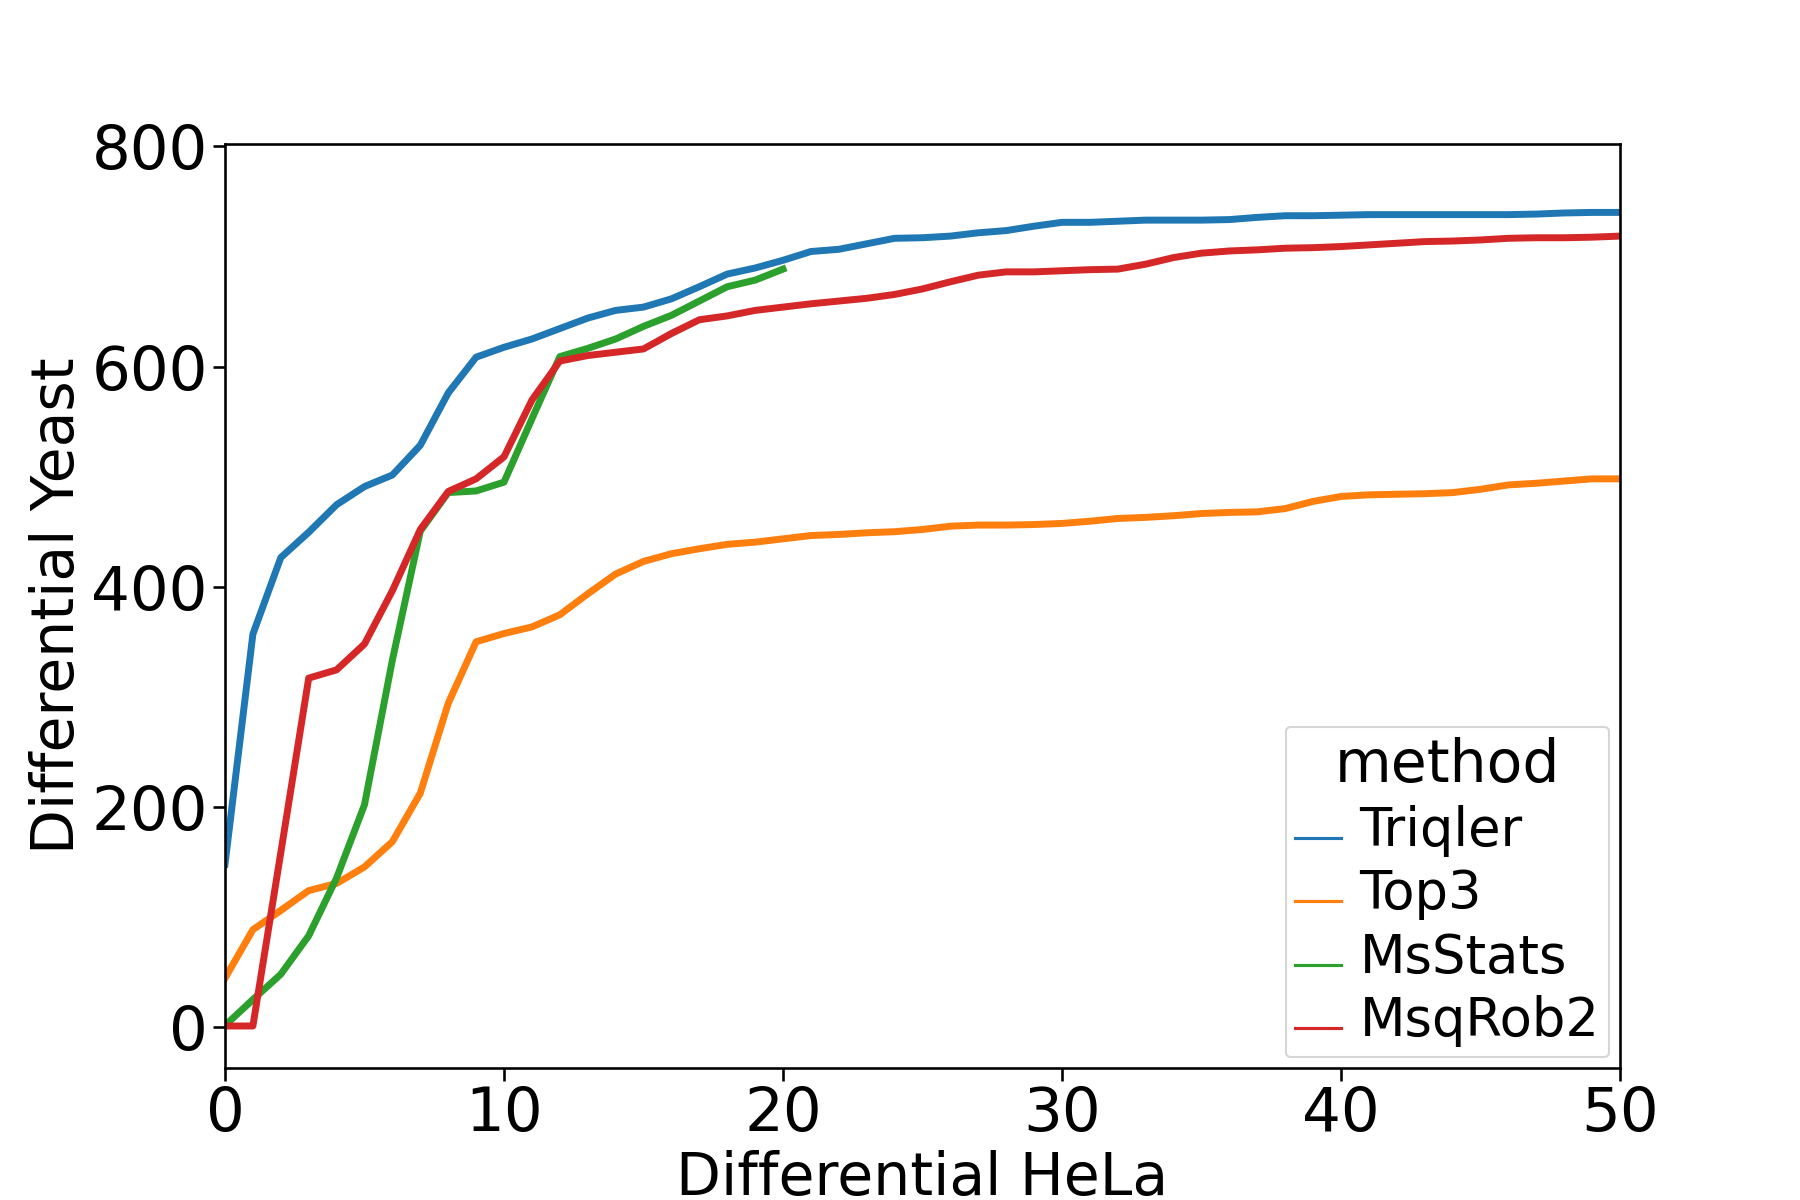
\includegraphics[width=0.4\linewidth]{../../result/report_plots_pipeline/diff_HeLa_vs_nonHeLa_PS_yeast_0.51.png} \\
        C & 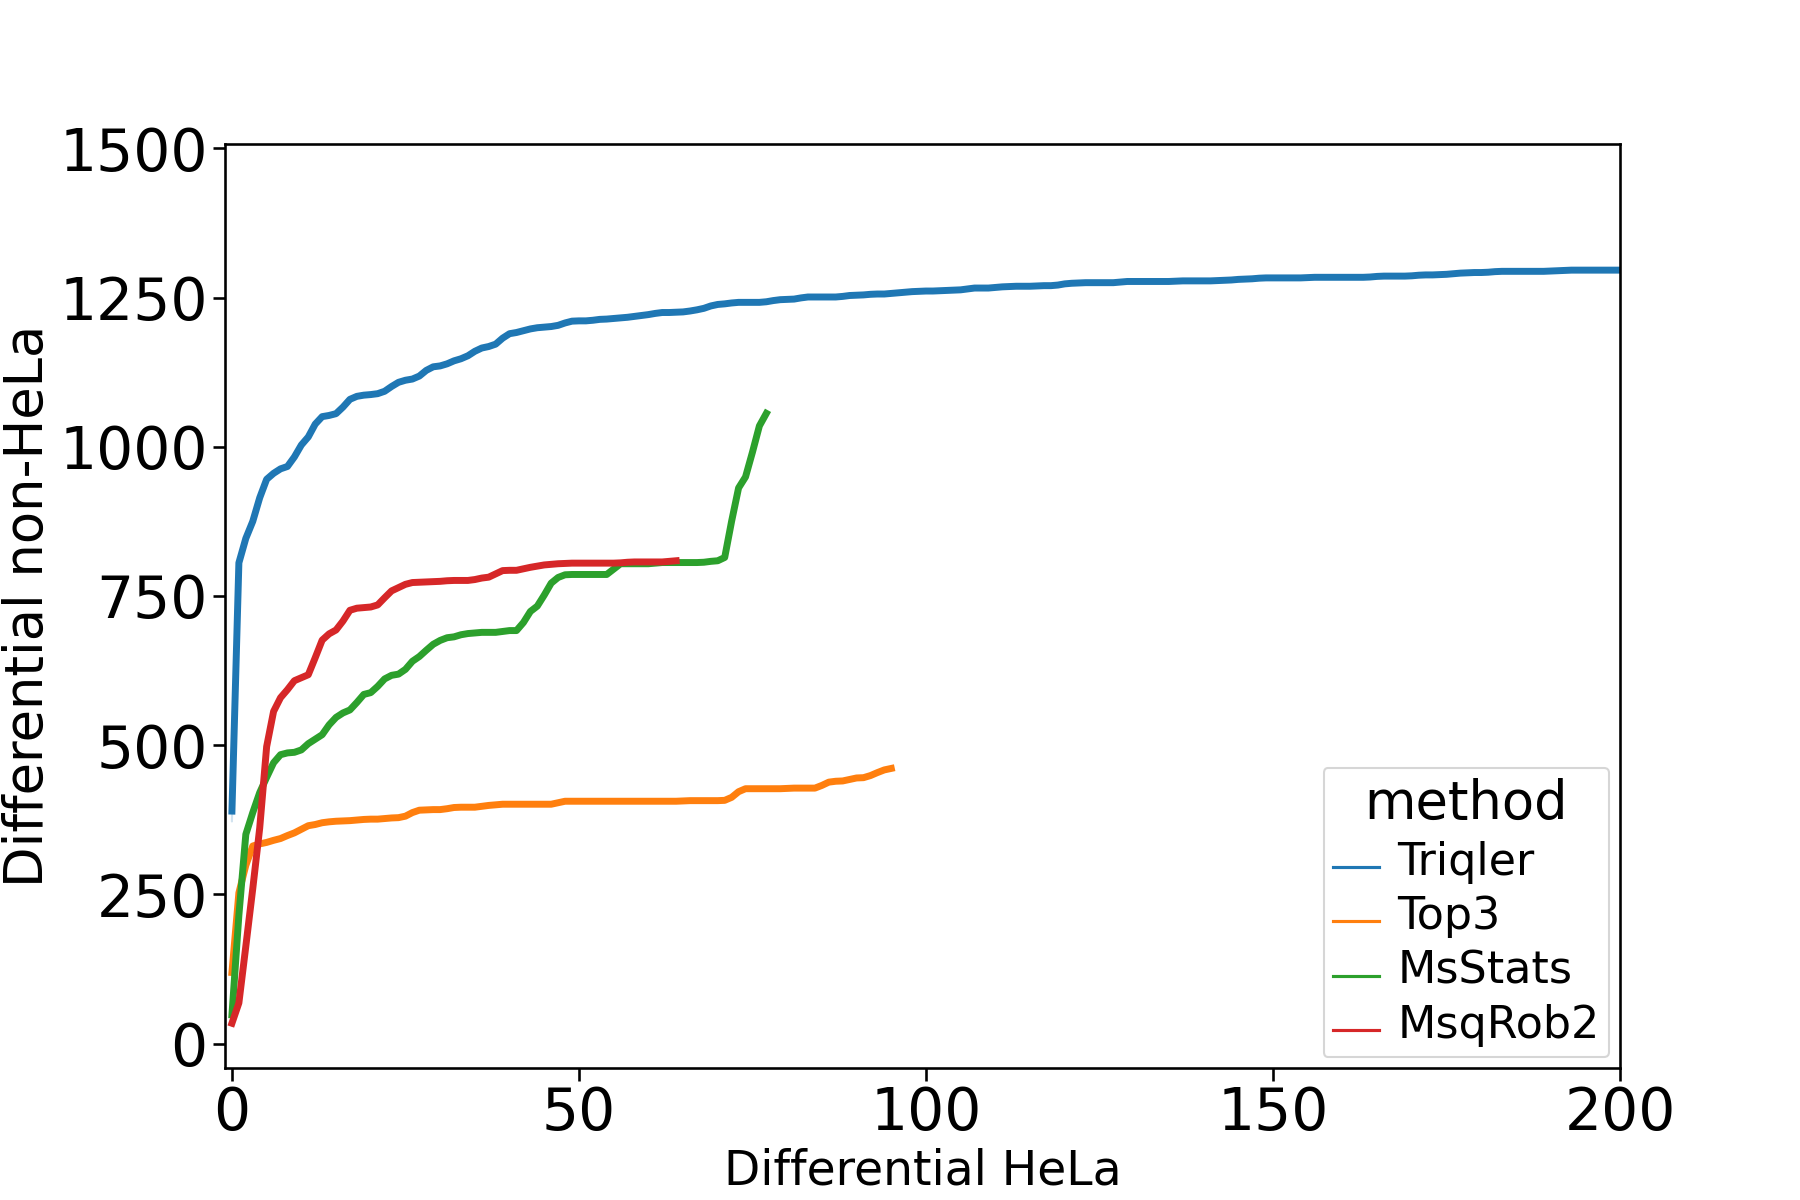
\includegraphics[width=0.4\linewidth]{../../result/report_plots_pipeline/diff_HeLa_vs_nonHeLa_ID_all_0.51.png} & 
        F & 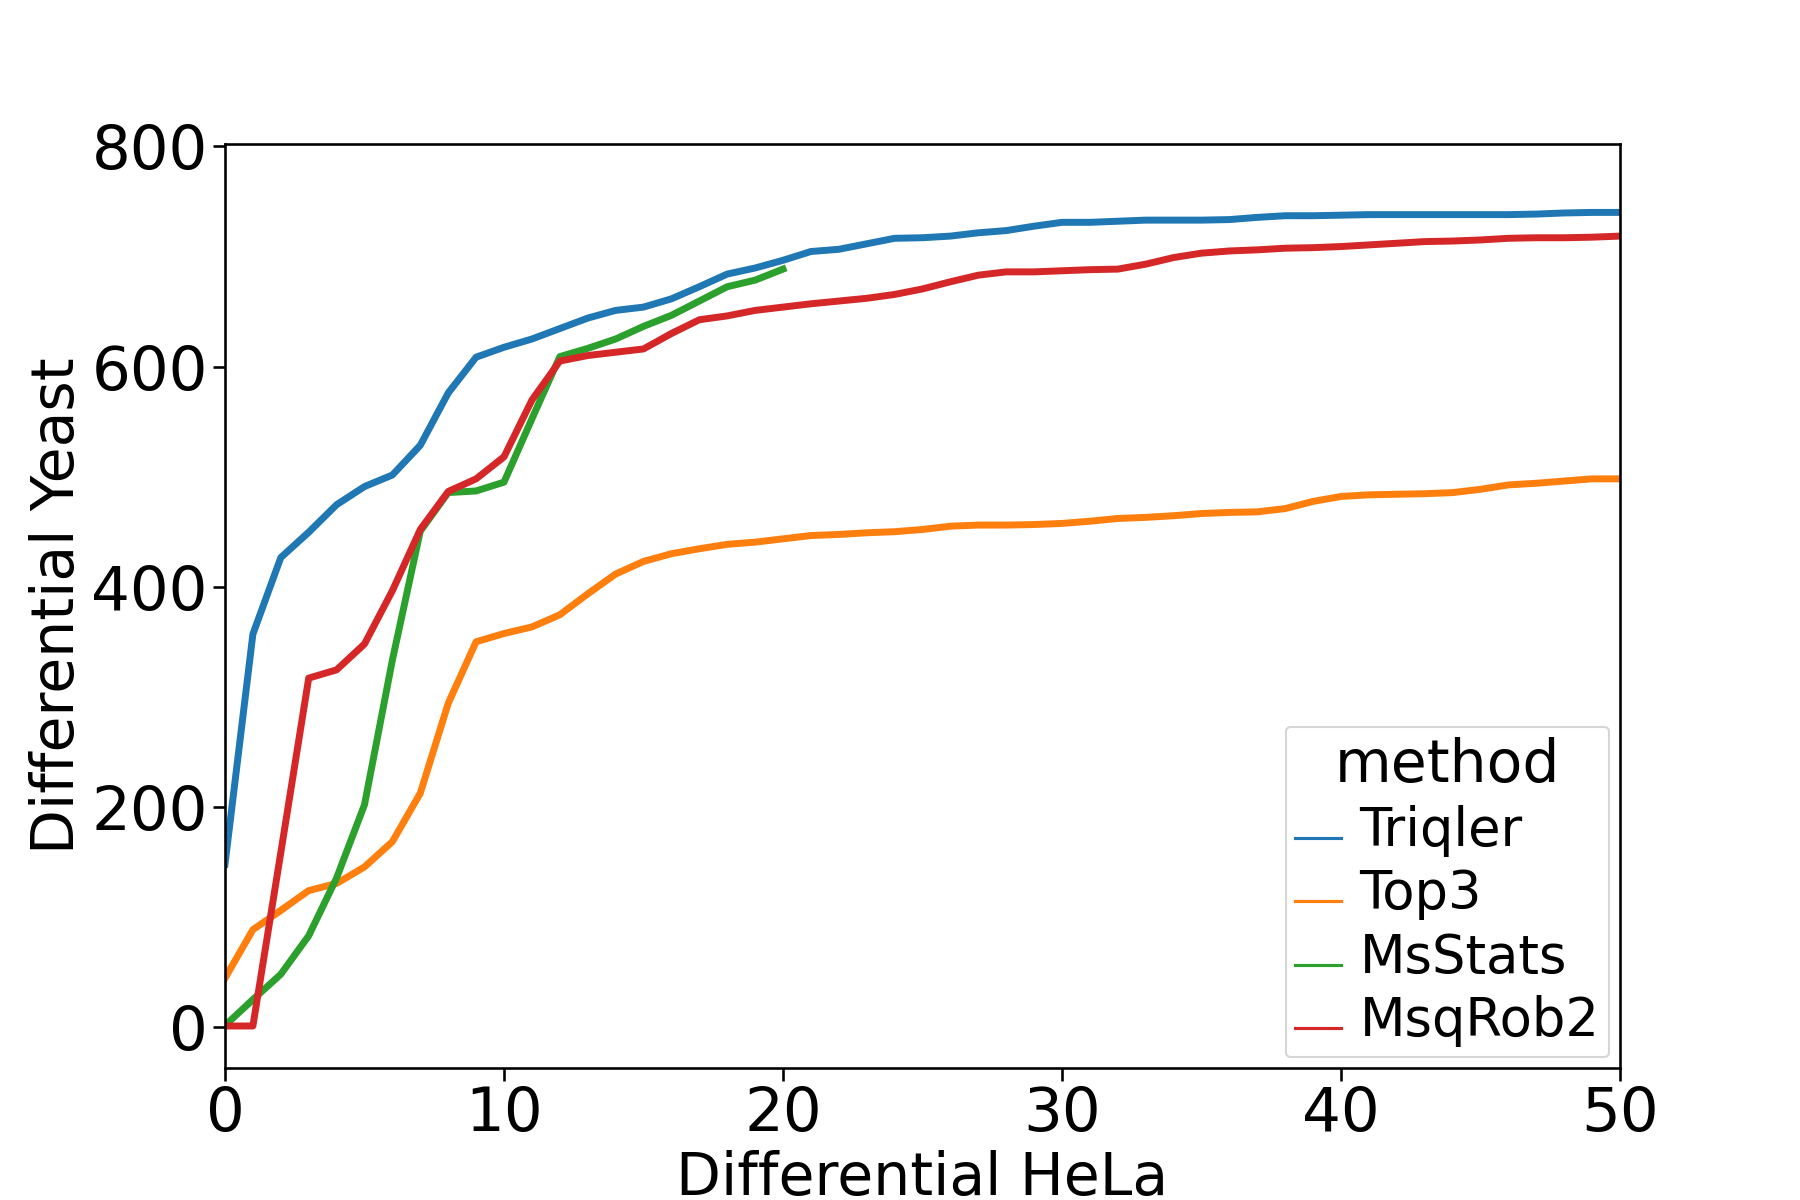
\includegraphics[width=0.4\linewidth]{../../result/report_plots_pipeline/diff_HeLa_vs_nonHeLa_PS_yeast_0.51.png} \\ 

    \end{tabular}
    \caption{{\bf The compared methods' ability to differentiate differentially abundant proteins.} We plotted the number of reported differentially abundant  {\em E. Coli} and Yeast proteins as a function of the number of proteins from the HeLa background when sorting according to significance for (A) ID pipeline and (B) PS pipeline. For the test, we selected a fold-change evaluation of 0.51 for Triqler and fold-change threshold of 0.51 for Top3, MSstats, and MSqRob2. All methods have a protein-level FDR threshold of 0.01. \label{fig:ability_to_differentiate_differentially_abundant_specie_vs_hela}}
\end{figure}


\begin{figure}[hbt]
    \centering
    \newcolumntype{V}{>{\centering\arraybackslash} m{.4\linewidth} }
    \setlength{\tabcolsep}{0pt}

    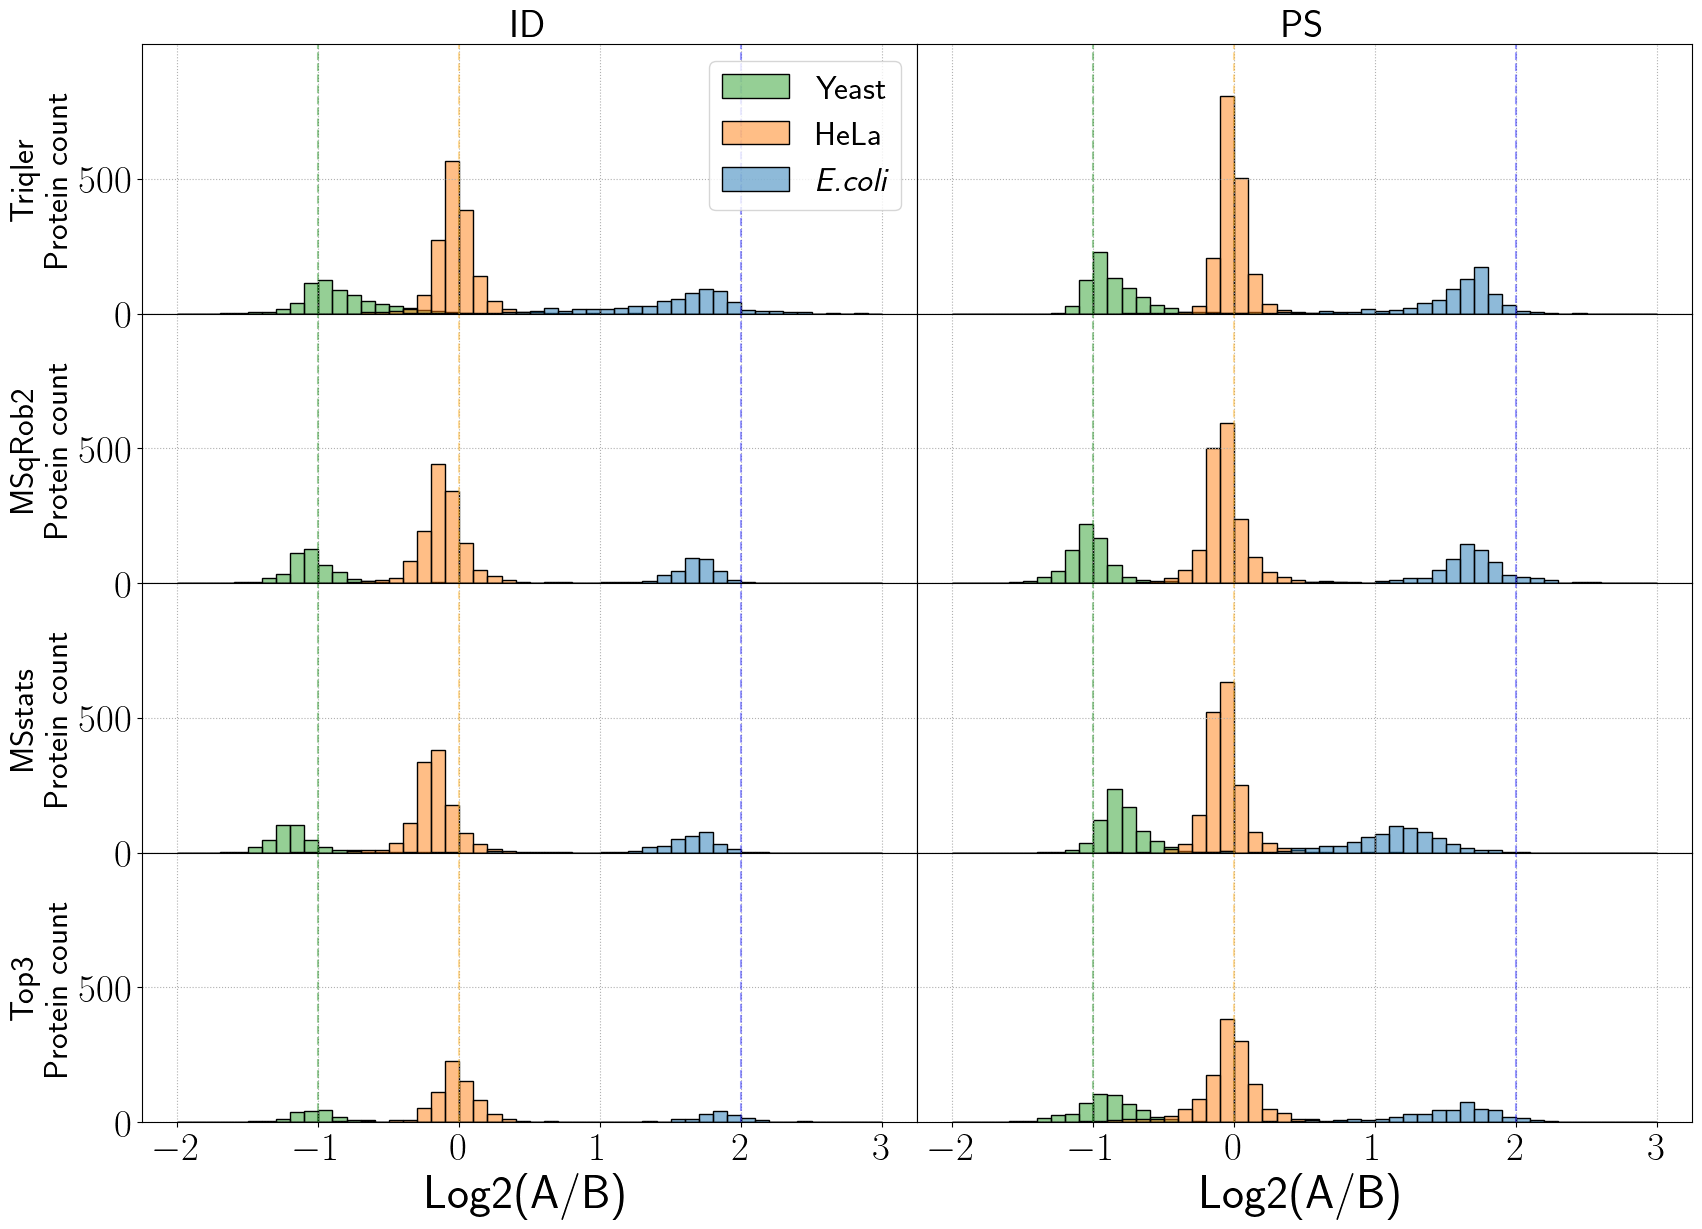
\includegraphics[width=\linewidth]{../../result/report_plots/gridplot_histogram.png} 


    \caption{{\bf Comparison of reported fold change distributions.} We can see that the Triqler and Top3 log2(A/B) empirical distributions have apexes that are more centered toward the true lysate values, which are indicated by the dashed lines. The apexes for Triqler have higher protein count than MSqRob2, MSstats and Top3. This shows that there are more proteins closer to the true values identified by Triqler than the other methods. \label{fig:fc_histogram_supplement}}
    \todo[inline]{Harmonize font sizes.}
    
\end{figure}


\begin{figure}[hbt]
    \centering
    \centering
    \begin{tabular}{c} 
        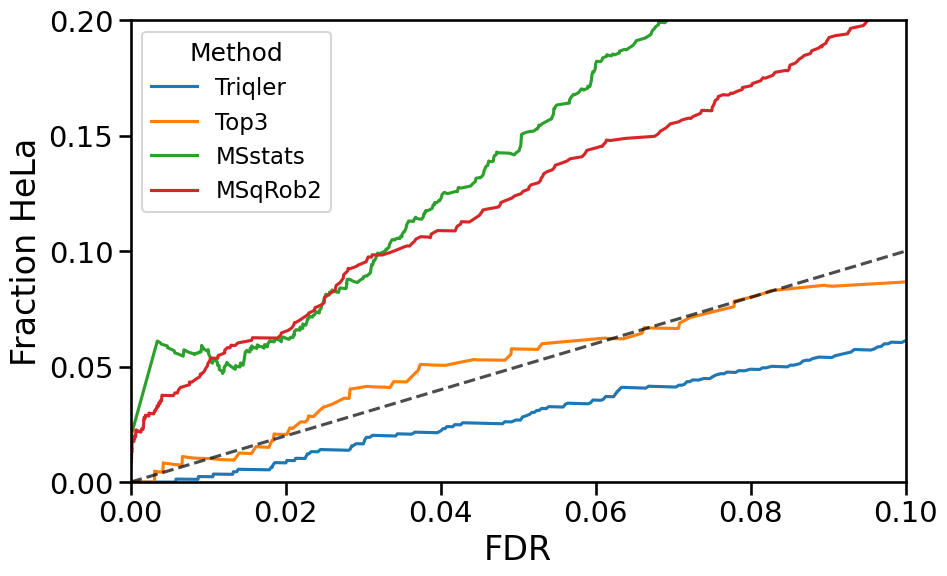
\includegraphics[width=0.5\linewidth]{../../result/report_plots_pipeline/calibration_ID_0.png} \\
        A \\ 
        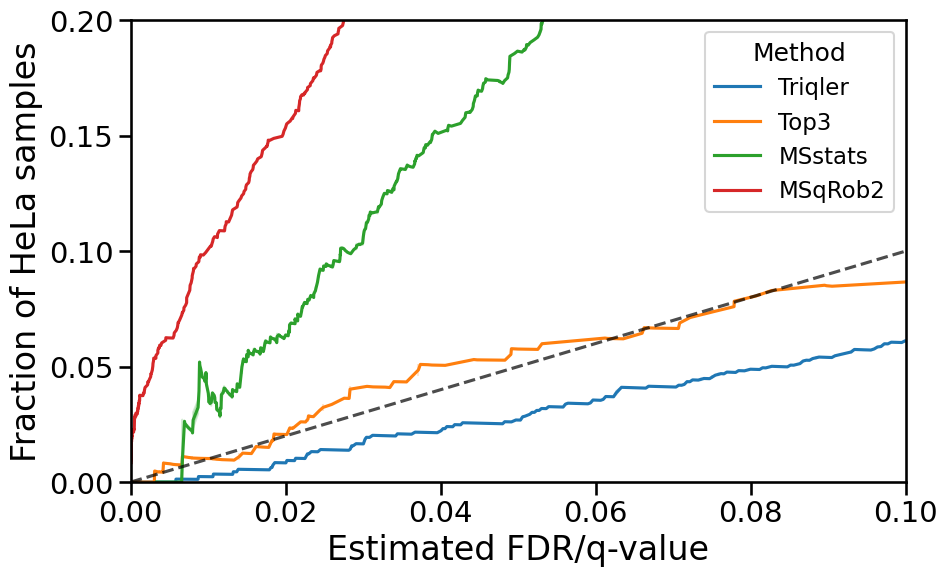
\includegraphics[width=0.5\linewidth]{../../result/report_plots_pipeline/calibration_ID_0.51.png} \\
        B \\
        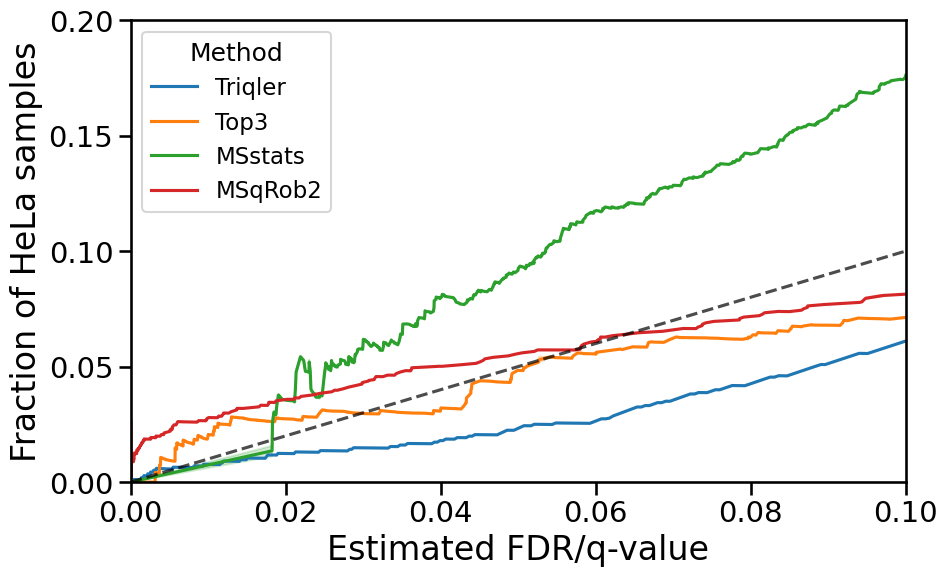
\includegraphics[width=0.5\linewidth]{../../result/report_plots_pipeline/calibration_PS_0.png} \\
        C \\
        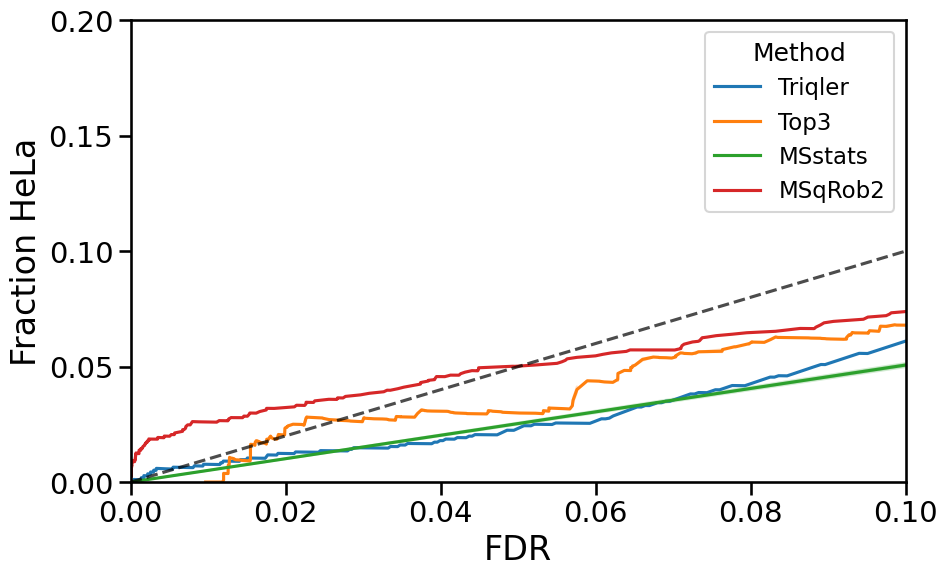
\includegraphics[width=0.5\linewidth]{../../result/report_plots_pipeline/calibration_PS_0.51.png} \\
        D 
    \end{tabular}
  \caption{{\bf Comparison of calibration of the compared summarization methods.} We plotted the fraction of reported differentially abundant HeLa proteins as a function of $q$~value for (A,B) ID pipeline and (C,D) PS pipeline. The non-Triqler estimated proteins abundances were both (A,C) not subject to fold change thresholds and (B,D) subject to a 0.51 fold change threshold. \label{fig:frac_hela_vs_fdr_supp}}
\end{figure}


\end{document}

